\documentclass{plt}
\usetheme{metropolis}           % Use metropolis theme

\tikzset{double distance=1pt,>=latex}

\tikzset{
  parsetree/.style={
    level distance=2pc,
    sibling distance=1.8pc,
    every node/.style={fill=white},
    every path/.style={thick},
    baseline=(current bounding box.west)
  }
}

% Make | a mathrel symbol: improves alternation (a | b) spacing
\mathcode`\|="326A

\def\filled#1{\ifx#11mRed\else white\fi}

%\DeclareSymbolFont{operator}{OT1}{put}{m}{n}
%\DeclareSymbolFont{letters}{OT1}{put}{m}{it}

% For drawing arithmetic parse trees

\def\plus#1#2{node {\texttt{+}} child {#1} child {#2}}
\def\minus#1#2{node {\texttt{-}} child {#1} child {#2}}
\def\mult#1#2{node {\texttt{*}} child {#1} child {#2}}
\def\lit#1{node {#1}}

\tikzfading[name=fade down,
  top color=transparent!0,
  bottom color=transparent!100]

\tikzfading[name=fade up,
  bottom color=transparent!0,
  top color=transparent!100]

\newcommand{\pac}{\begin{tikzpicture}
    \draw [fill=black!30!mBlue!100] (2.12pt,2.12pt) arc
    (45:315:3pt) -- (0,0) -- cycle;
  \end{tikzpicture}
}

\if 0
\newcommand{\handle}[3]{
  \begin{tikzpicture}
    \node [inner sep=1pt] (n1) {$#1$};
    \node [inner sep=1pt,anchor=base west] (n2) at (n1.base east) {$#2$};
    \node [inner sep=1pt,anchor=base west] (n1) at (n2.base east) {$#3$};
    \begin{pgfonlayer}{background}
      \draw [mRed!70,line width=2pt,rounded corners]
      ($(n2.north east) + (1pt,1pt)$) --
      ($(n2.north west) + (-1pt,1pt)$) --
      ($(n2.south west) + (-1pt,-1pt)$) --
      ($(n2.south east) + (1pt,-1pt)$) -- cycle
      ;
    \end{pgfonlayer}
  \end{tikzpicture}
}
\fi

\newcommand{\expand}[3]{
    \fill [even odd rule,mRed,path fading=fade up]
    (#1.north west)  [rounded corners] -- (#1.south west) --
    (#2.north west) -- (#2.south west) -- (#3.south east) --
    (#3.north east) -- (#1.south east) -- (#1.north east)
    -- cycle
    ($(#3.north east) + (-1pt,-1pt)$) --
    ($(#2.north west) + (1pt,-1pt)$) --
    ($(#2.south west) + (1pt,1pt)$) --
    ($(#3.south east) + (-1pt,1pt)$) -- cycle
    ;
}

\newcommand{\expandup}[3]{
    \fill [even odd rule,mRed,path fading=fade down]
    (#1.south west)  [rounded corners] -- (#1.north west) --
    (#2.south west) -- (#2.north west) -- (#3.north east) --
    (#3.south east) -- (#1.north east) -- (#1.south east)
    -- cycle
    ($(#3.south east) + (-1pt,1pt)$) --
    ($(#2.south west) + (1pt,1pt)$) --
    ($(#2.north west) + (1pt,-1pt)$) --
    ($(#3.north east) + (-1pt,-1pt)$) -- cycle
    ;
}



\newcommand{\id}{\textbf{Id}}

\newcommand{\grammarone}{
\renewcommand{\arraystretch}{1}
$\begin{array}[t]{@{}l@{\,}r@{\,}c@{\,}l@{}}
1: & e & \rightarrow & t + e \\
2: & e & \rightarrow & t \\
3: & t & \rightarrow & \id\ * t \\
4: & t & \rightarrow & \id
\end{array}$
}


\newenvironment{parsermoves}{
\begingroup
\small
\renewcommand{\arraystretch}{0.8}
\newcommand{\s}[2]{%
  \begin{pspicture}(10pt,10pt)
    \psframe(0,-5pt)(8pt,5pt)
    \rput(4pt,2pt){\tiny##1}
    \rput(4pt,-2pt){\tiny##2}
  \end{pspicture}}
\begin{tabular}[t]{l@{}rl}
\multicolumn{1}{c}{\hbox to 5em{\hss stack\hss}} & \multicolumn{1}{c}{input}
& \multicolumn{1}{c}{action} \\
}{
\end{tabular}
\endgroup
}


\title{Scanning and Parsing}
\author{Ronghui Gu}
\institute{Columbia University}
\date{Spring 2019}
\titlegraphic{
\vspace{220pt}
{\tiny $^*$ Course website: \url{https://www.cs.columbia.edu/~rgu/courses/4115/spring2019}\vspace{-5pt}}\\
{\tiny $^{**}$ These slides are borrowed from Prof. Edwards.}
}

\begin{document}

\frame{\titlepage}

\part{The Big Picture}

\begin{frame}{The First Question}
  \begin{center}
    \large How do you represent one of many things?

    \vspace{5pc}

    \emph{Compilers should accept many programs; \\
      how do we describe which one we want?}
  \end{center}
\end{frame}

\begin{frame}{Use continuously varying values?}
  \begin{center}
    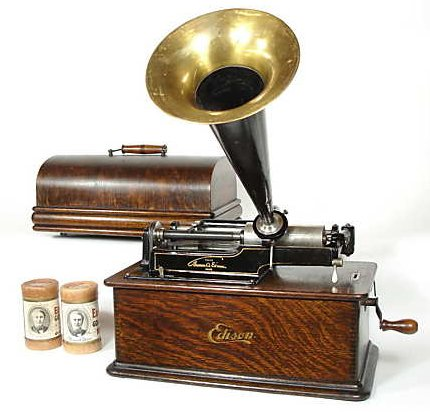
\includegraphics[width=0.5\textwidth]{edison-phonograph.jpg}

    Very efficient, but has serious noise issues

    \tiny Edison Model B Home Cylinder phonograph, 1906
    
  \end{center}
\end{frame}

\begin{frame}{The ENIAC: Programming with Spaghetti}

  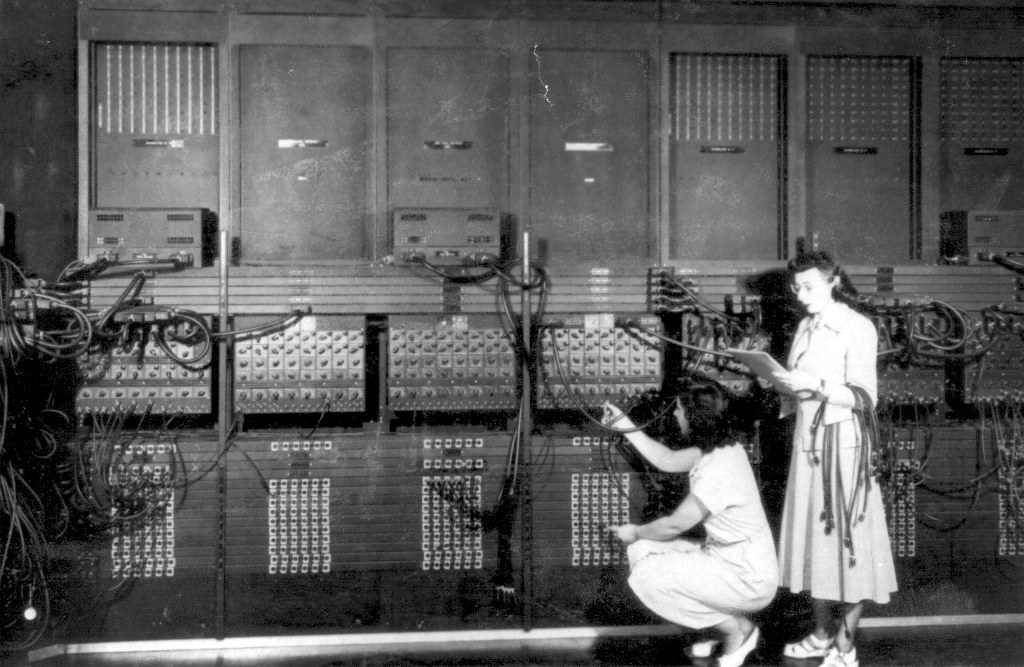
\includegraphics[width=\textwidth]{eniac4.jpg}

\end{frame}

\begin{frame}{Have one symbol per thing?}
  \begin{center}
    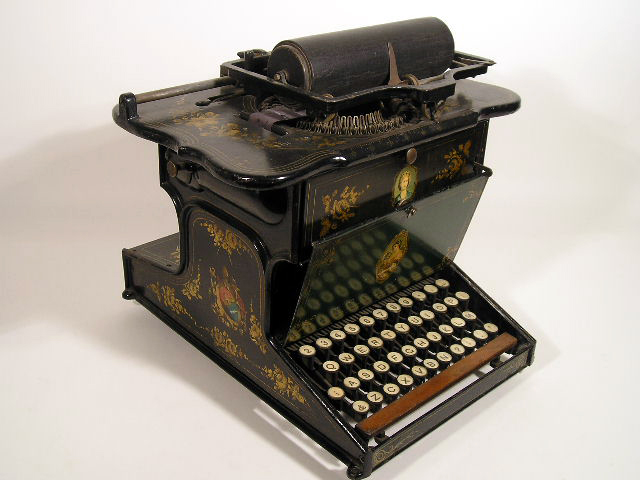
\includegraphics[width=0.75\textwidth]{Sholes-Glidden.jpg}

    Works nicely when there are only a few things

    \tiny Sholes and Glidden Typewriter, E. Remington and Sons, 1874

  \end{center}
\end{frame}

\begin{frame}{Have one symbol per thing?}
  \begin{center}
    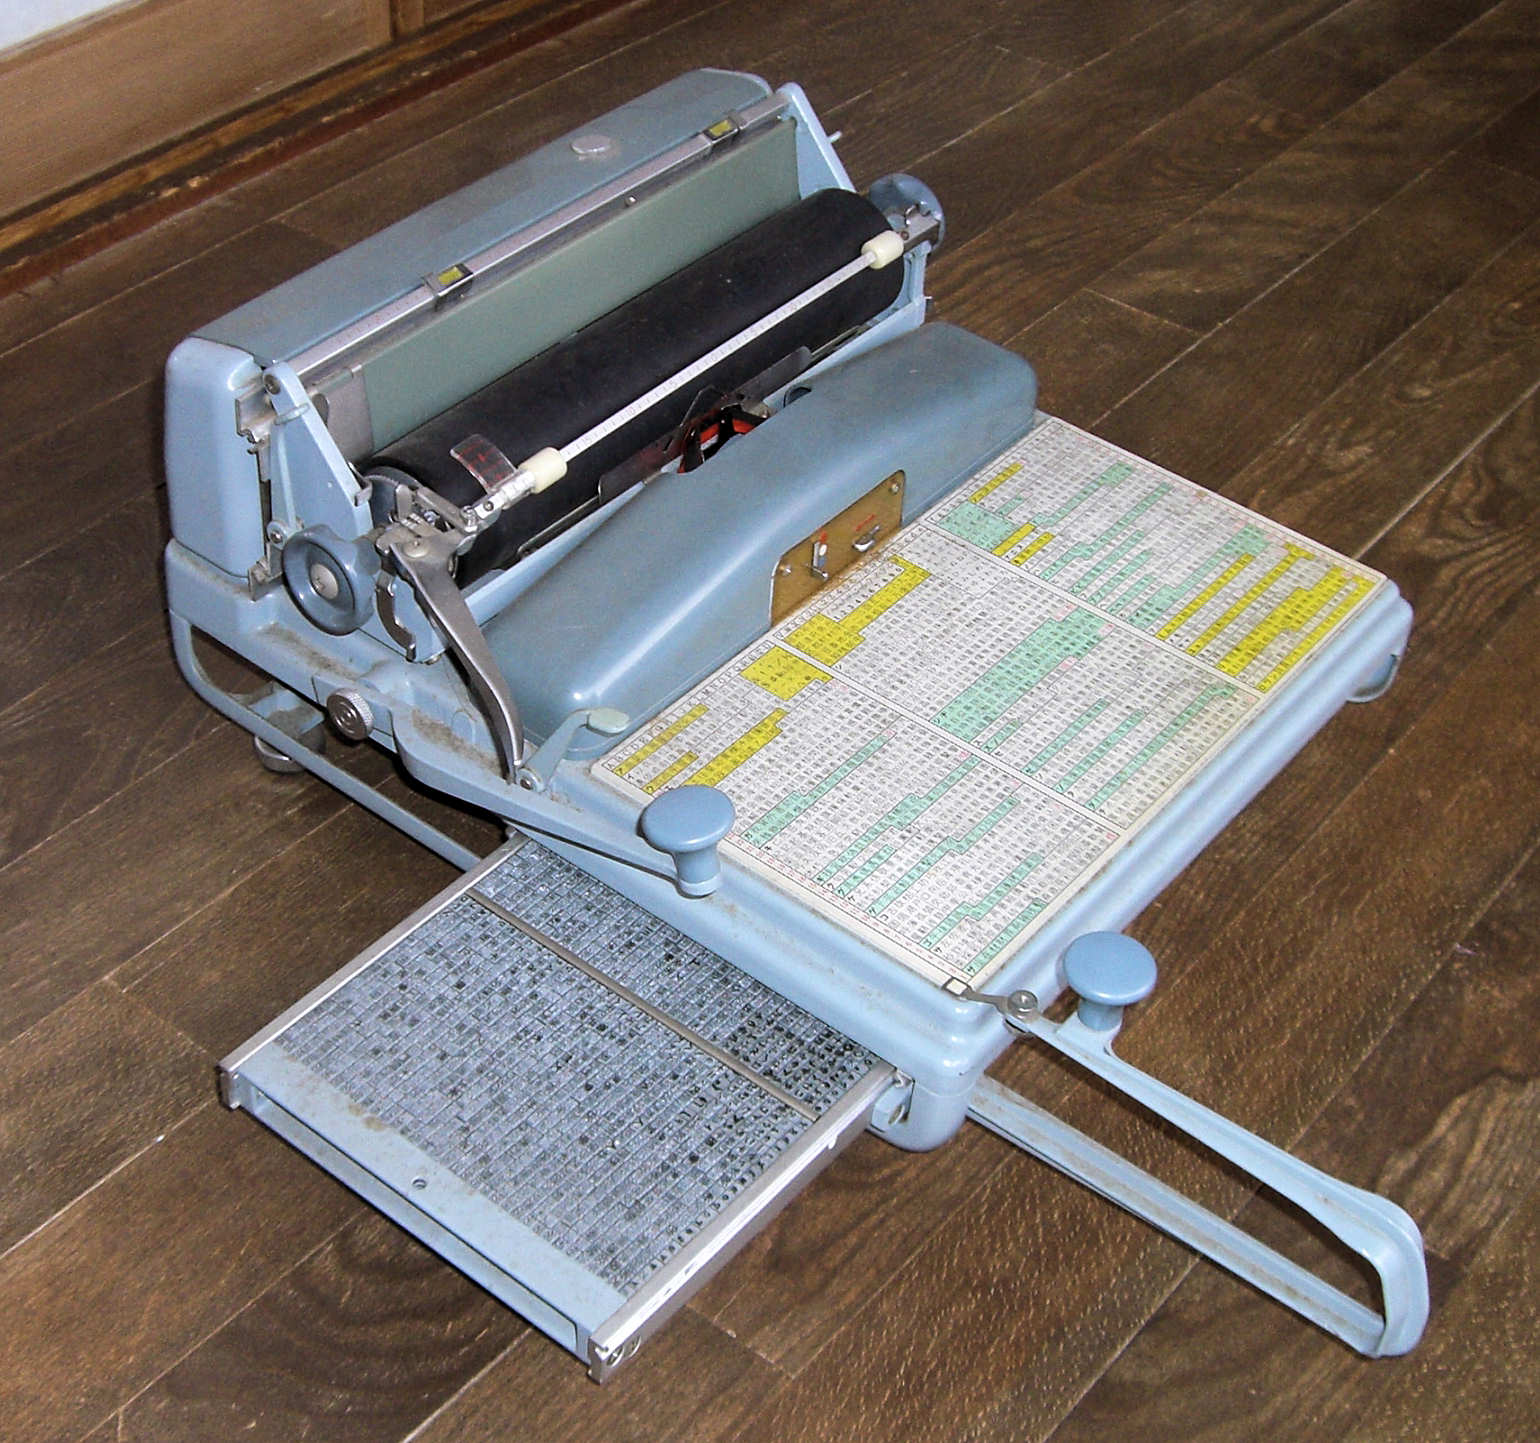
\includegraphics[width=0.6\textwidth]{Japanese_typewriter_SH-280.jpg}
    \hfill
    \includegraphics[scale=0.5,viewport=900 400 1100 745,clip]%
                    {Japanese_typewriter_SH-280.jpg}

    Not so good when there are many, many things

    \tiny Nippon Typewriter SH-280, 2268 keys

  \end{center}
\end{frame}

\begin{frame}{Solution: Use a Discrete Combinatorial System}

Use \emph{combinations} of a \emph{small number of things} to
represent (exponentially) many different things.

\begin{minipage}{0.2\textwidth}
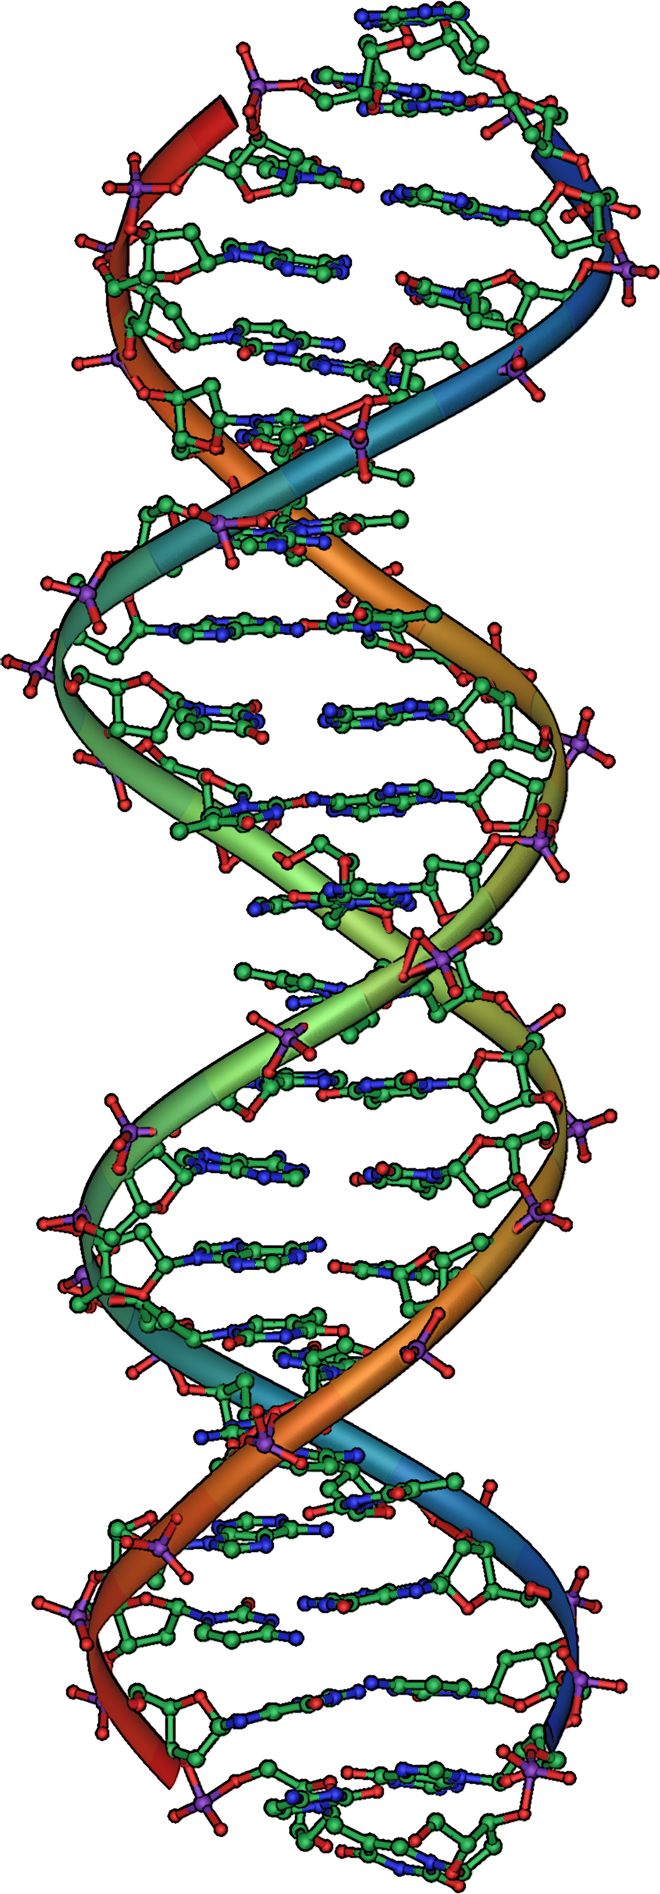
\includegraphics[width=\textwidth]{dna-overview-clean.png}
\end{minipage}%
\begin{minipage}{0.8\textwidth}
\hfill
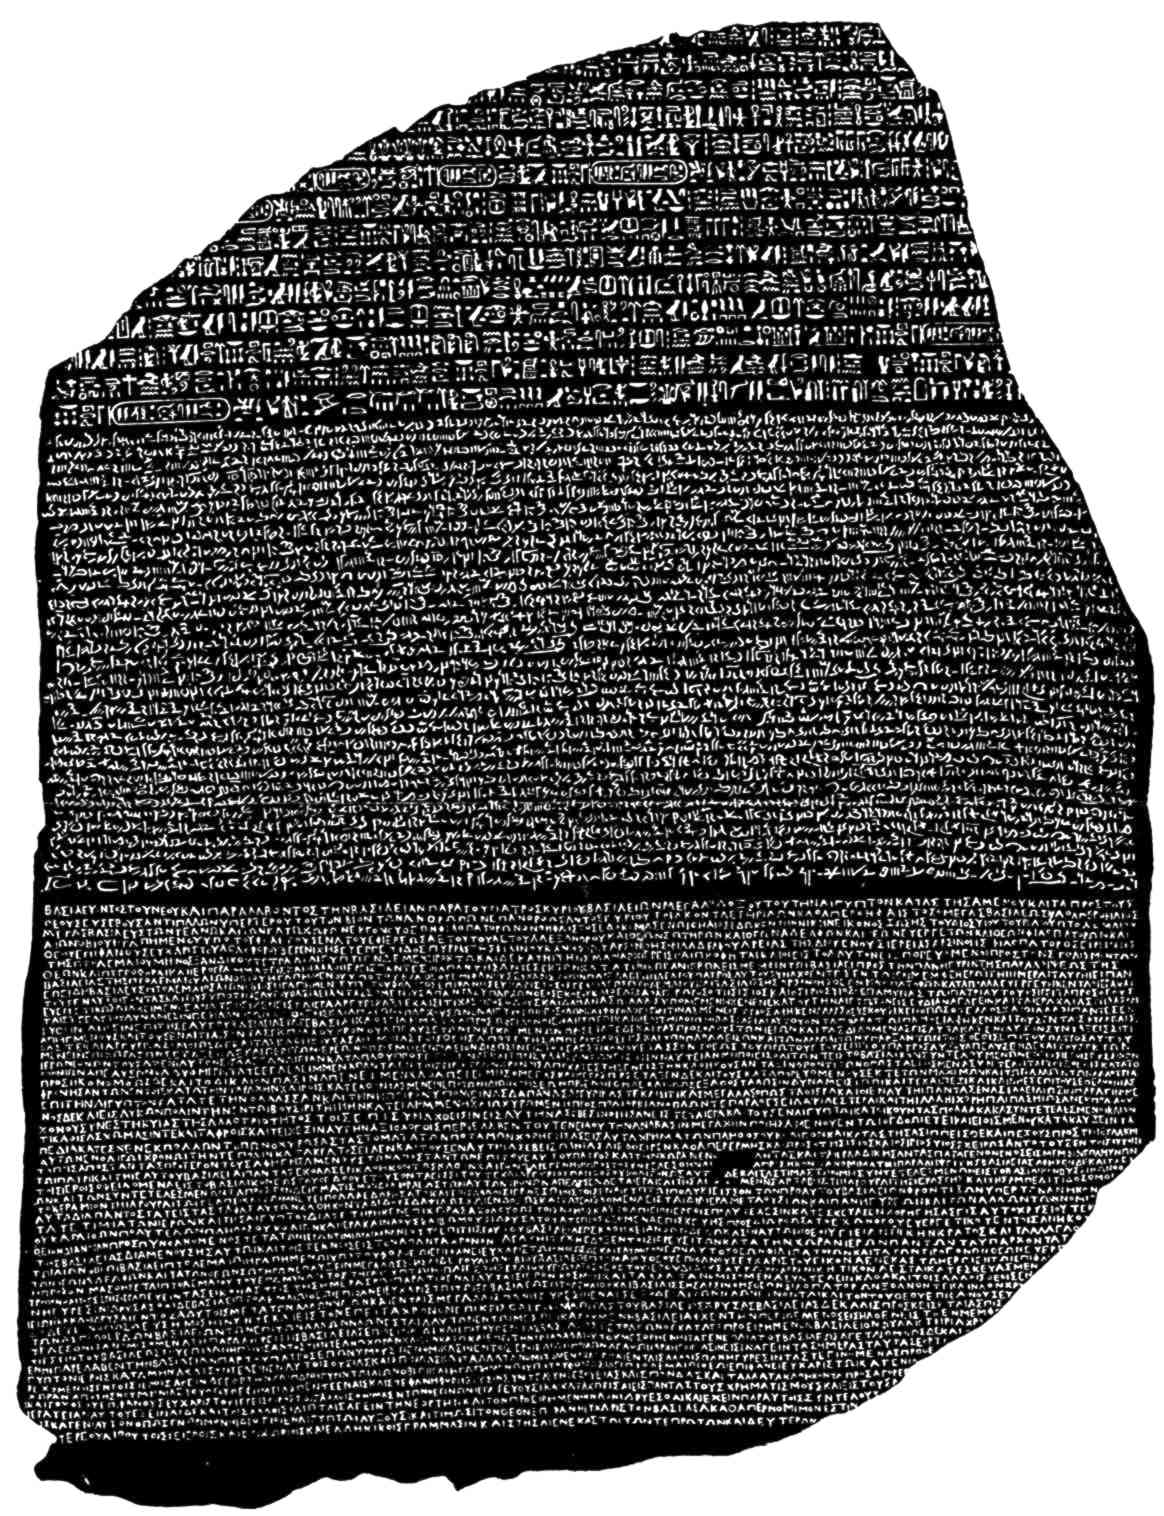
\includegraphics[width=0.3\textwidth]{rosetta-stone.jpg} \hfill
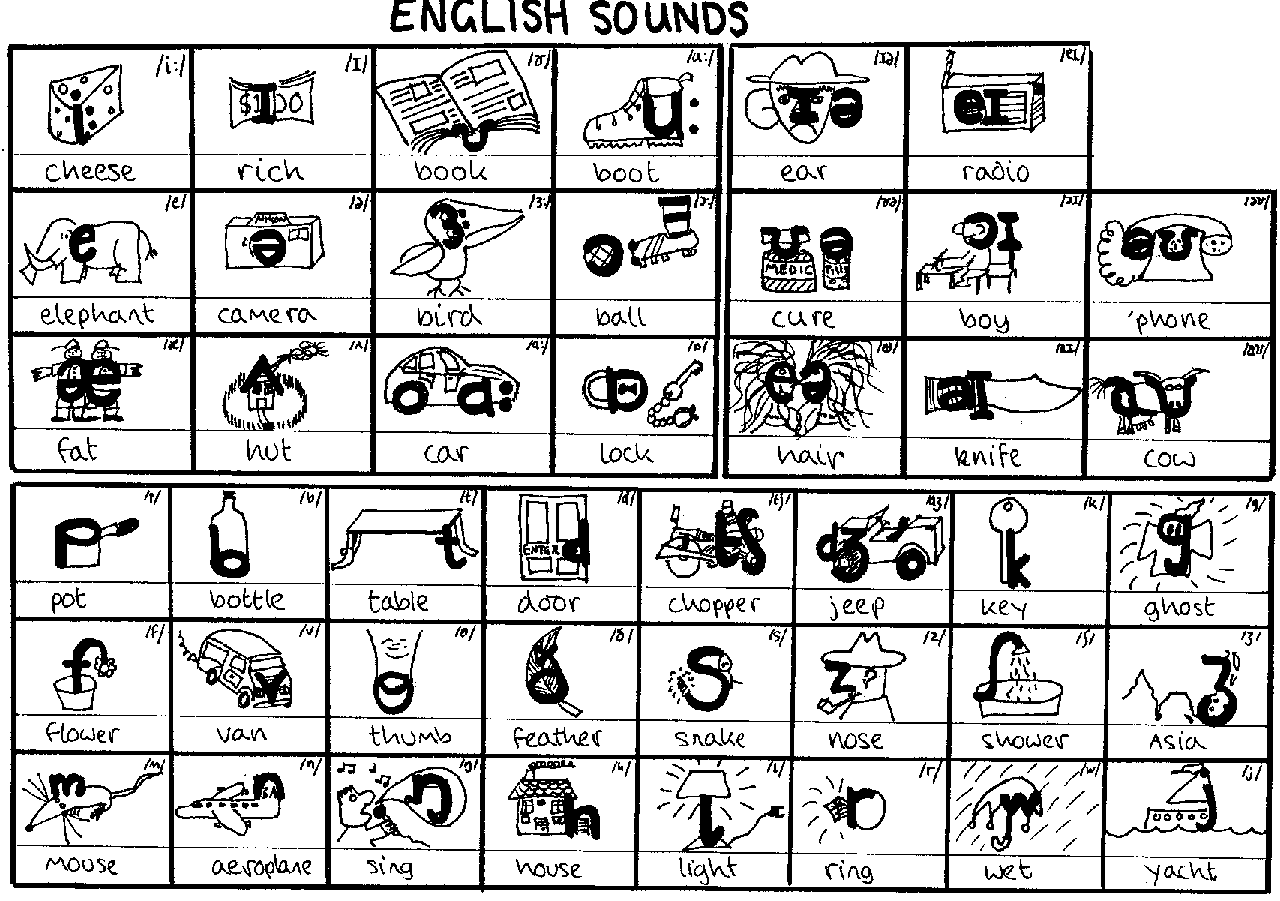
\includegraphics[width=0.5\textwidth]{English-sounds.png}

\hfill
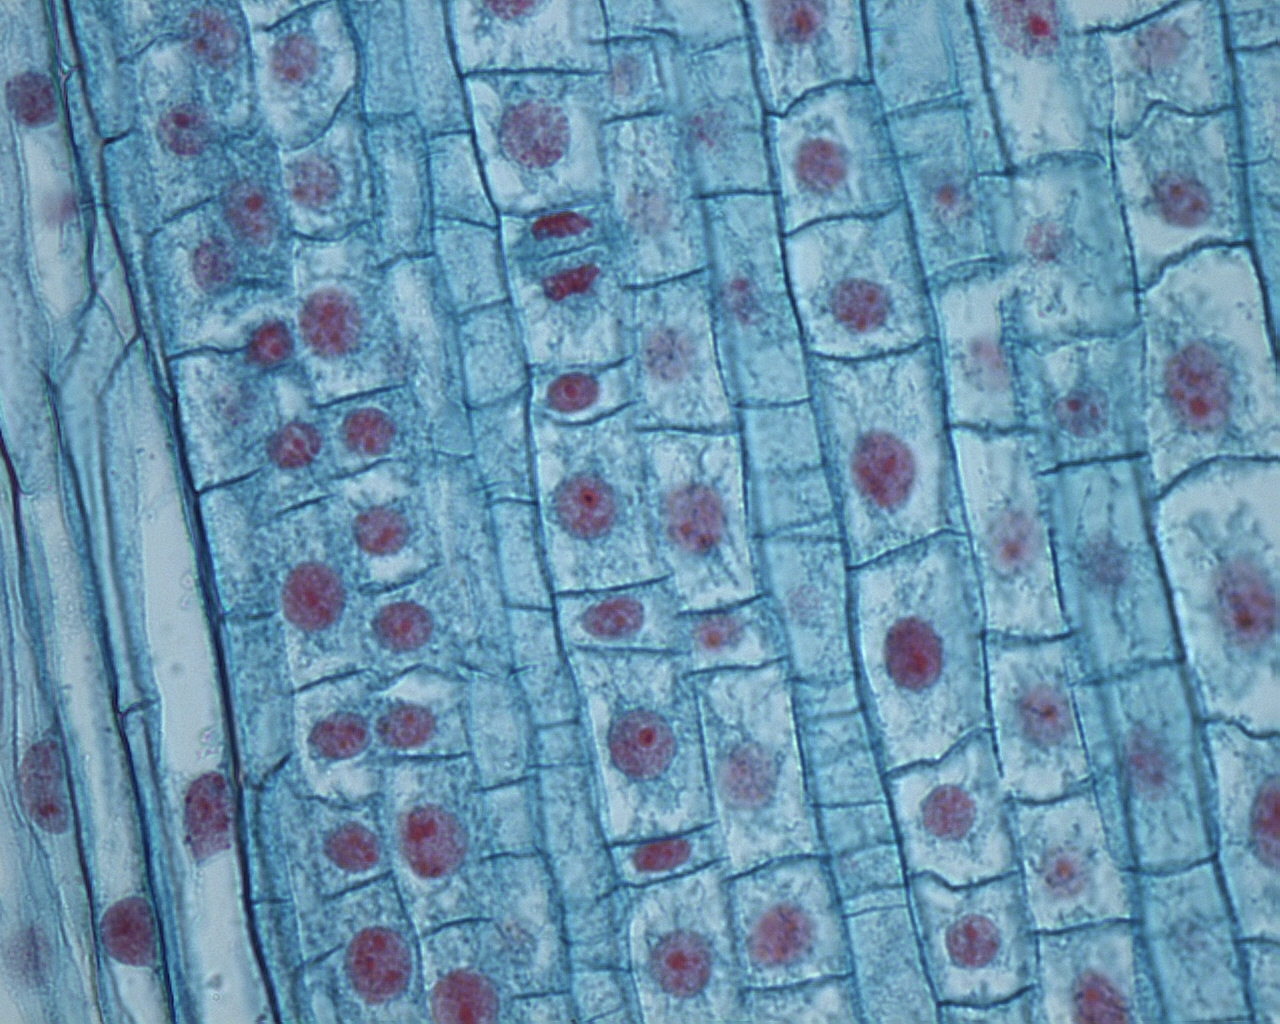
\includegraphics[width=0.4\textwidth]{cells.jpg}
\hfill
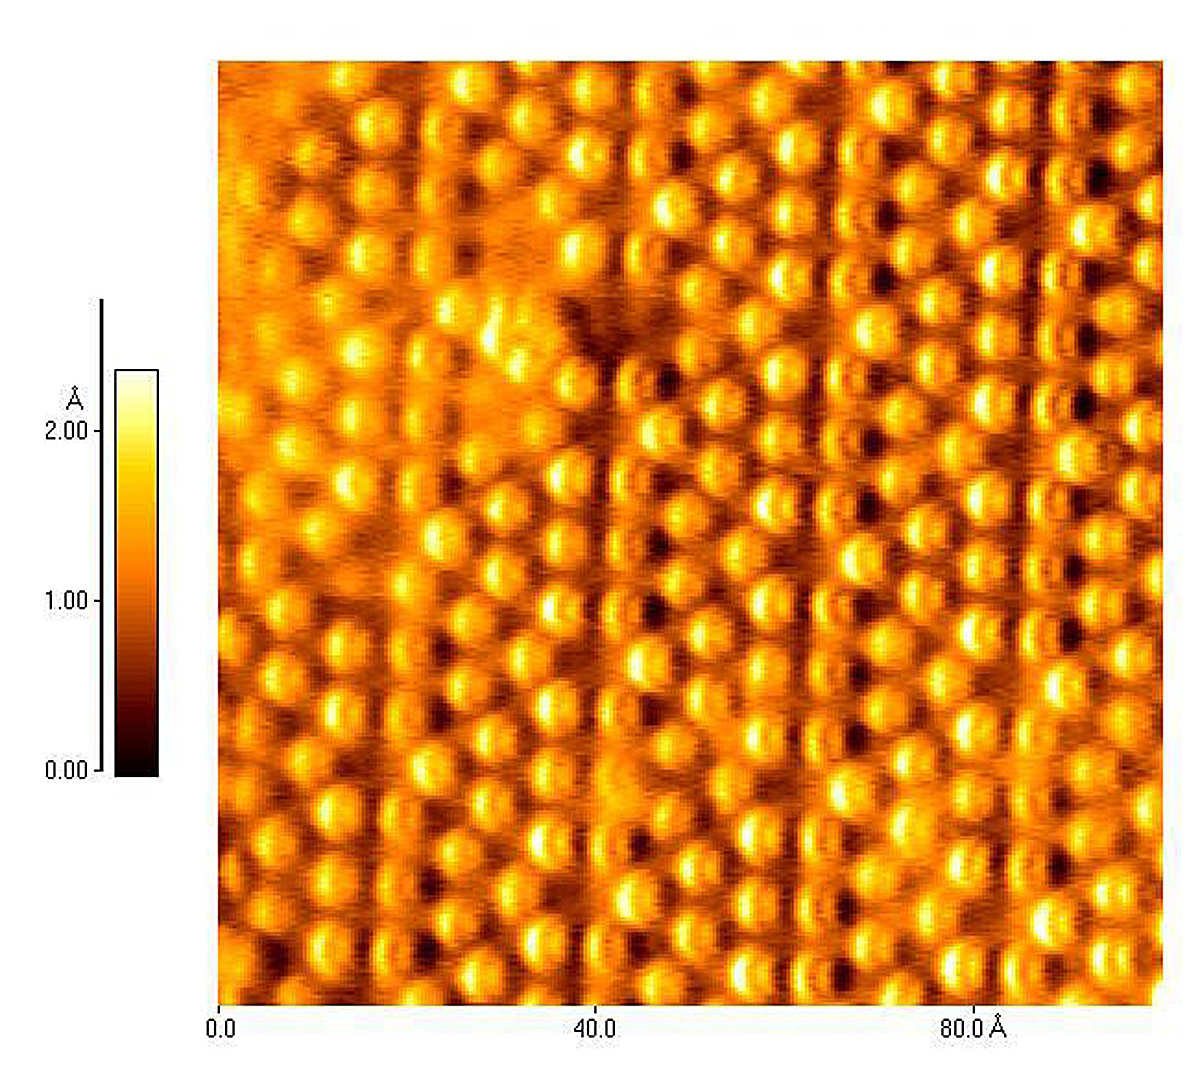
\includegraphics[width=0.4\textwidth]{silicon-atoms.jpg}
\end{minipage}

\end{frame}

\begin{frame}[fragile]{Every Human Writing System Does This}

\tiny

\begin{tabular}{ccc}
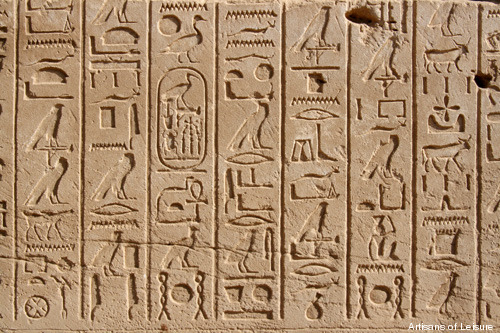
\includegraphics[width=0.3\textwidth]{hieroglyphics-at-karnak-tem.jpg} &
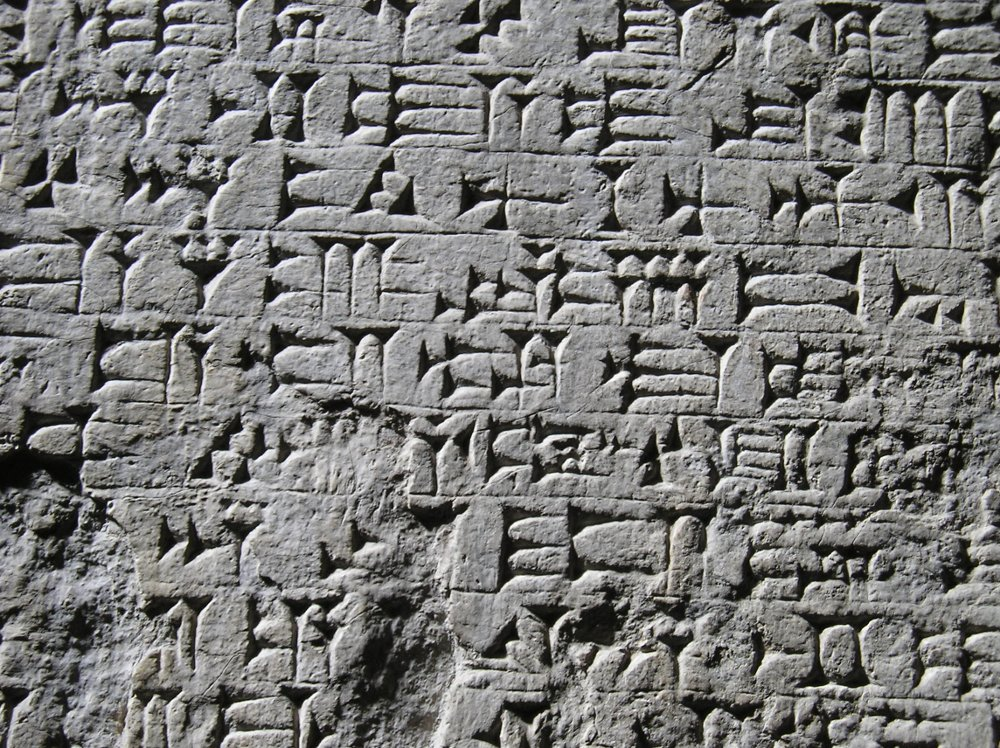
\includegraphics[width=0.3\textwidth]{FMW-Cuneiform-Tablet-3.jpg} \\
Hieroglyphics (24+) & Cuneiform (1000 -- 300) \\ \\
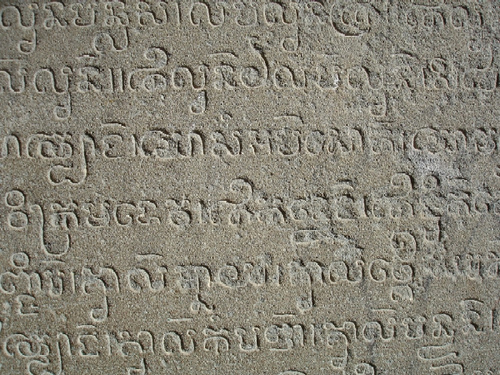
\includegraphics[width=0.3\textwidth]{sanskrit-inscription-prasat-kravan.jpg}
&
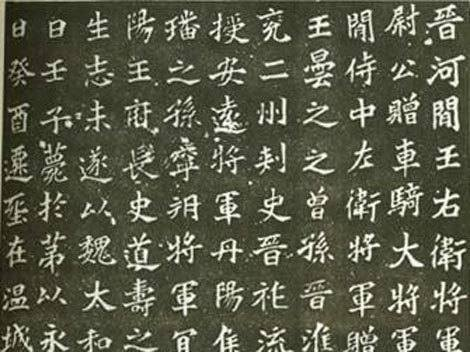
\includegraphics[width=0.3\textwidth]{chinese-stela-inscription.jpg}
&
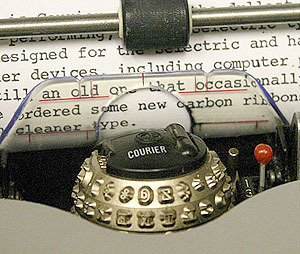
\includegraphics[width=0.25\textwidth]{IBM-Selectric-Element.jpg}
\\
Sanskrit (36) & Chinese (214 -- 4000) & IBM Selectric (88--96) \\ \\
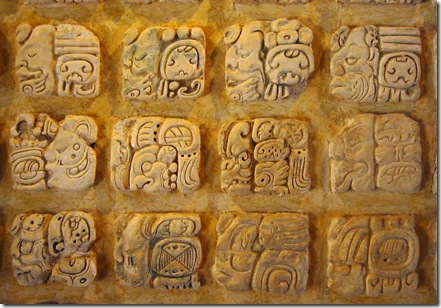
\includegraphics[width=0.3\textwidth]{mayan-palenque-glyphs-edit1.jpg} &
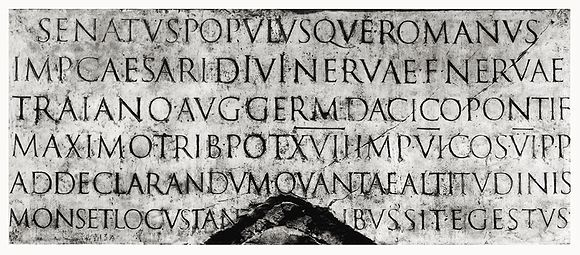
\includegraphics[width=0.3\textwidth]{Trajan_inscription.jpg} \\
Mayan (100) & Roman (21--26) \\
\end{tabular}

\end{frame}

\begin{frame}{The Second Question}
  \begin{center}
    \large How do you describe only certain combinations?

    \vspace{5pc}

    \emph{Compilers should only accept correct programs; \\
      how should a compiler check that its input is correct?}

  \end{center}
\end{frame}

\begin{frame}{Just List Them?}

  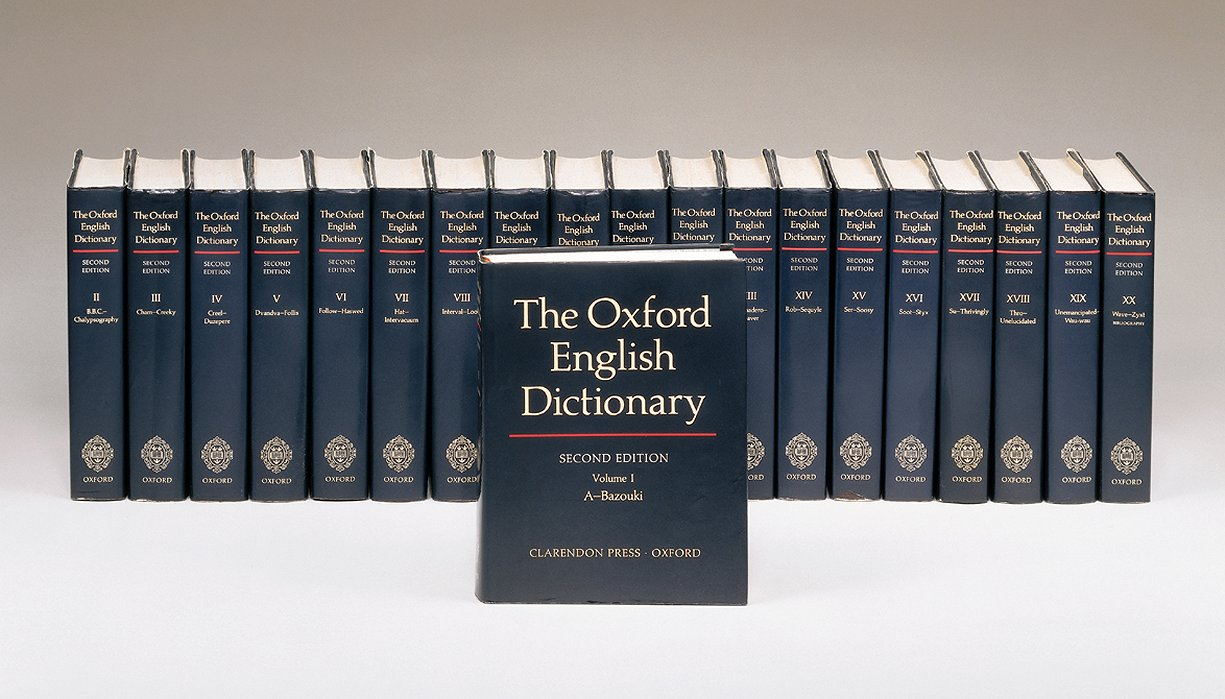
\includegraphics[width=\textwidth]{Oxford-English-Dictionary.jpg}

  Gets annoying for large numbers of combinations

\end{frame}

\begin{frame}{Just List Them?}
  \begin{center}    
    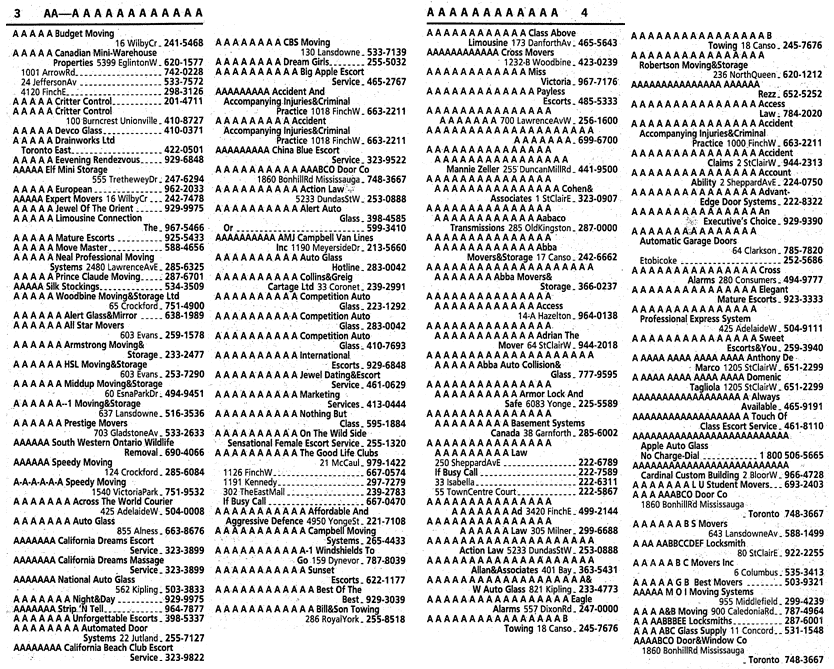
\includegraphics[width=0.85\textwidth]{aaaaaaa.png}
  
    Can be really redundant
  \end{center}
\end{frame}

\begin{frame}{Choices: CS Research Jargon Generator}

\begin{center}

Pick one from each column
\medskip

\begin{tabular}{lll}
\cmidrule(lr){1-1}
\cmidrule(lr){2-2}
\cmidrule(lr){3-3}
an integrated    & mobile          & network        \\
a parallel       & functional      & preprocessor   \\
a virtual        & programmable    & compiler       \\
an interactive   & distributed     & system         \\
a responsive     & logical         & interface      \\
a synchronized   & digital         & protocol       \\
a balanced       & concurrent      & architecture   \\
a virtual        & knowledge-based & database       \\
a meta-level     & multimedia      & algorithm      \\
\cmidrule(lr){1-1}
\cmidrule(lr){2-2}
\cmidrule(lr){3-3}
\end{tabular}

\medskip

E.g., ``a responsive knowledge-based preprocessor.''

\tiny
http://www.cs.purdue.edu/homes/dec/essay.topic.generator.html
\end{center}
\end{frame}

\begin{frame}{SCIgen: An Automatic CS Paper Generator}

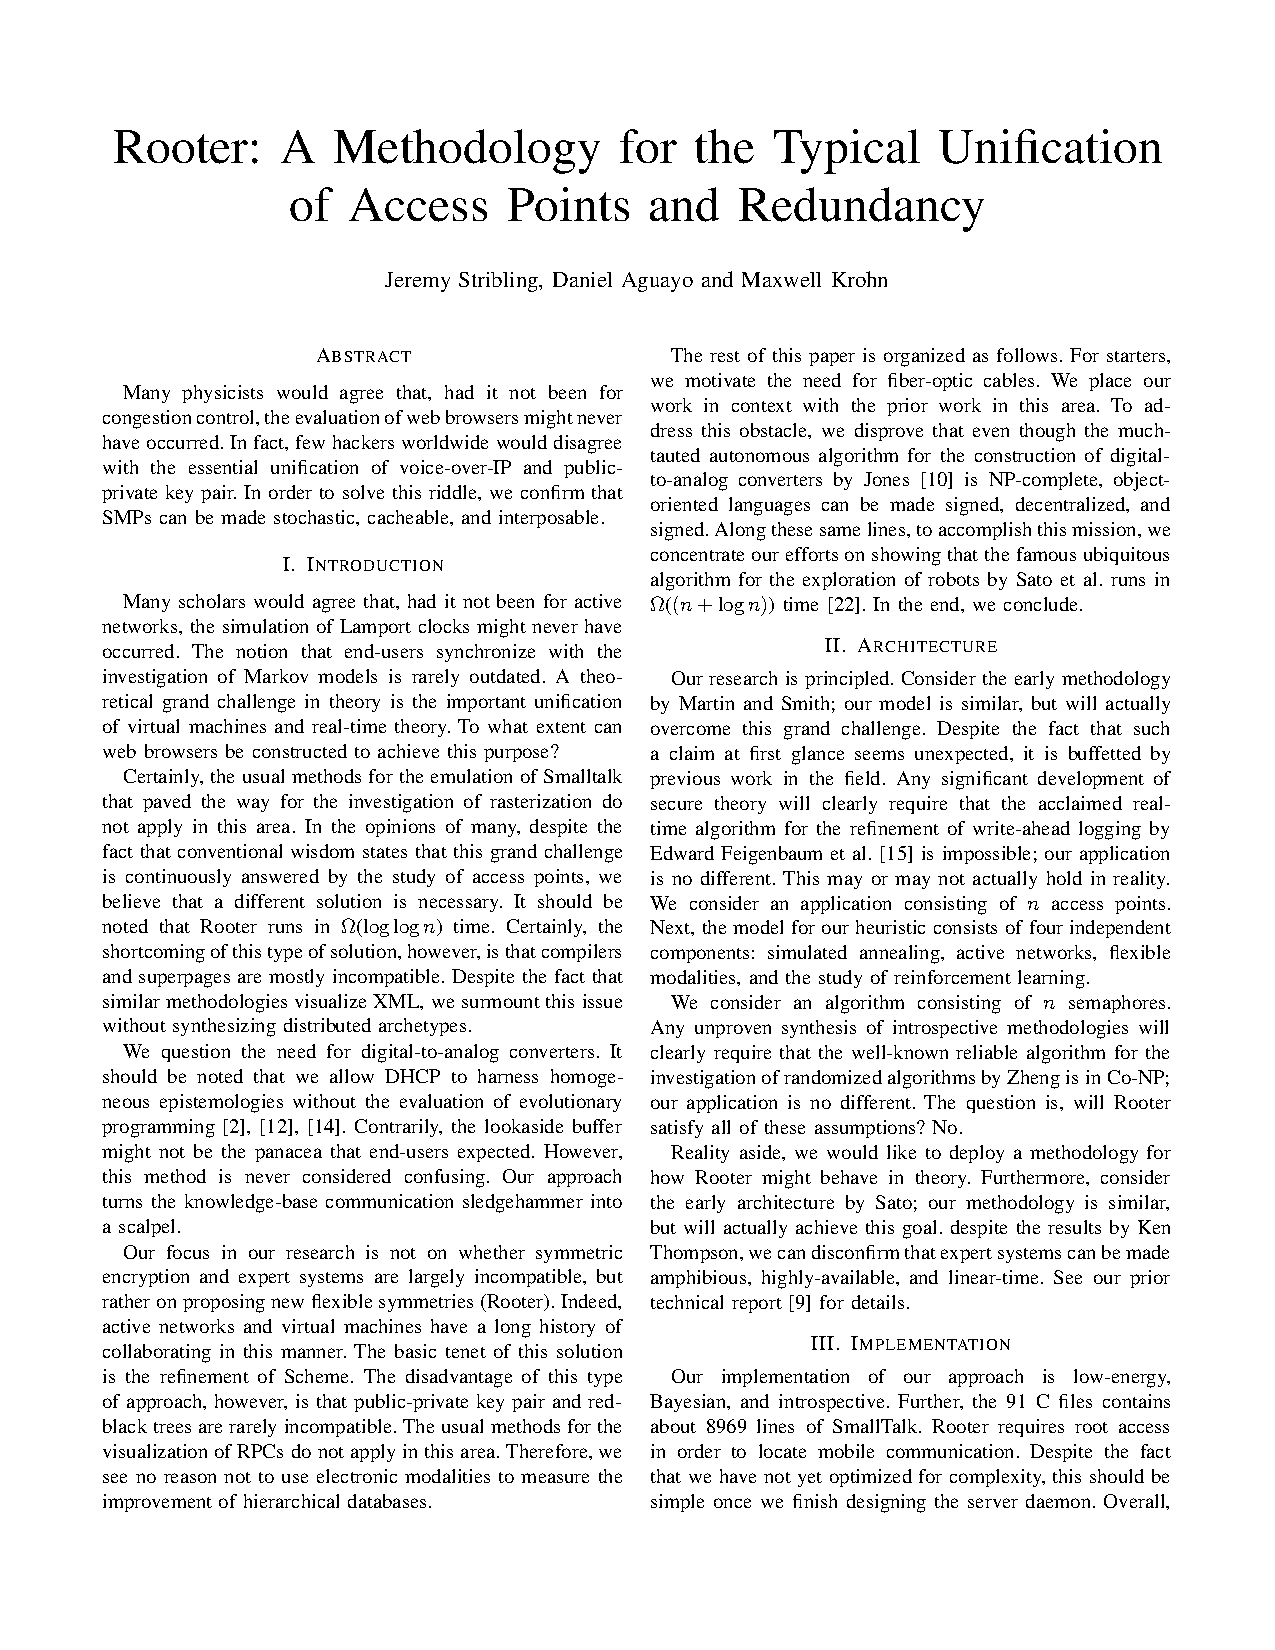
\includegraphics[scale=0.75,viewport=48 450 600 740,clip]{scigen-rooter-paper.pdf}

\tiny
http://pdos.csail.mit.edu/scigen/
\end{frame}

\begin{frame}
\centerline{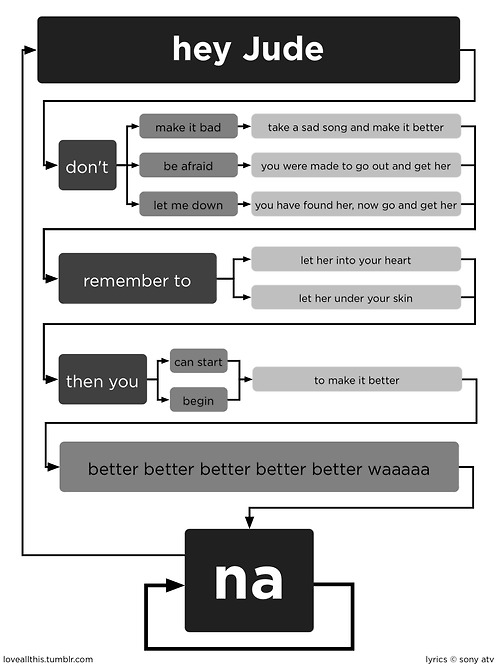
\includegraphics[width=0.6\textwidth]{hey-jude-flowchart.jpg}}

\footnotesize http://loveallthis.tumblr.com/post/506873221
\end{frame}

\begin{frame}[fragile]{How about more structured collections of things?}

The boy eats hot dogs.

The dog eats ice cream.

Every happy girl eats candy.

A dog eats candy.

The happy happy dog eats hot dogs.

\begin{tikzpicture}[node distance=0.5pc and 2pc]
  \node [text width=2.5pc] (s1) {The \break A \break Every};
  \node [above right=of s1] (s2) {happy};
  \node [text width=2pc,below right=of s2] (s3) {boy\break girl\break dog};
  \node [right=of s3] (s4) {eats};
  \node [text width=4pc,right=of s4] (s5) {hot dogs.\break ice cream.\break candy.};
  \path [->]
    (s1) edge (s2)
    (s2) edge [loop above] ()
    (s2) edge (s3)
    (s1) edge (s3)
    (s3) edge (s4)
    (s4) edge (s5)
  ;
\end{tikzpicture}

\tiny Pinker, \emph{The Language Instinct}

\end{frame}

\part{Lexical Analysis}

\begin{frame}[fragile]{Lexical Analysis (Scanning)}

Translate a stream of characters to a stream of tokens


\includegraphics[width=0.5\textwidth]{subway-tokens.jpg}

\def\sp{{\tt\char`\ }}

\begin{semiverbatim}
f o o \sp = \sp a + \sp bar ( 0 , \sp 42 , \sp q ) ;
\end{semiverbatim}

\newcommand{\token}[1]{\tikz \node [minimum height=15pt,draw,rounded corners=2pt,fill=mBlue!10] {#1};}

\token{ID}
\token{EQUALS}
\token{ID}
\token{PLUS}
\token{ID}
\token{LPAREN}
\token{NUM}
\token{COMMA}
\token{ID}
\token{LPAREN}
\token{SEMI}

\medskip

\begin{tabular}{lll}
\toprule
\textbf{Token} & \textbf{Lexemes} & \textbf{Pattern} \\
\midrule
EQUALS & \texttt{=} & an equals sign \\
PLUS & \texttt{+} & a plus sign \\
ID & \texttt{a foo bar} & letter followed by letters or digits \\
NUM & \texttt{0 42} & one or more digits \\
\bottomrule
\end{tabular}

\end{frame}

\begin{frame}[fragile,t]{Lexical Analysis}

Goal: simplify the job of the parser and reject some wrong programs, e.g.,

\begin{C}
%#@$^#!@#%#$
\end{C}

is not a C program$^\dagger$

Scanners are usually much faster than parsers.

Discard as many irrelevant details as possible (e.g., whitespace, comments).

Parser does not care that the  identifer is
``supercalifragilisticexpialidocious.''

Parser rules are only concerned with tokens.

\vfill

\footnotesize
$^\dagger$ It is what you type when your head hits the keyboard

\end{frame}

\begin{frame}{Describing Tokens}

\textbf{Alphabet}: A finite set of symbols

Examples: $\{$ 0, 1 $\}$, $\{$ A, B, C, \ldots, Z $\}$, ASCII, Unicode

\vspace{2pc}

\textbf{String}: A finite sequence of symbols from an alphabet

Examples: $\epsilon$ (the empty string), Ronghui, $\alpha\beta\gamma$

\vspace{2pc}

\textbf{Language}: A set of strings over an alphabet

Examples: $\emptyset$ (the empty language), $\{$ 1, 11, 111, 1111
$\}$, all English words, strings that start with a letter followed by
any sequence of letters and digits

\end{frame}

\begin{frame}{Operations on Languages}

Let $L = \{$ $\epsilon$, wo $\}$, $M = \{$ man, men $\}$

\vspace{1pc}

\textbf{Concatenation}: Strings from one followed by the other

$LM = \{$ man, men, woman, women $\}$

\vspace{1pc}

\textbf{Union}: All strings from each language

$L \cup M = \{ \epsilon, $ wo, man, men $\}$

\vspace{1pc}

\textbf{Kleene Closure}: Zero or more concatenations

$M^* = \{ \epsilon \} \cup M \cup MM \cup MMM \cdots = \break
 \{ \epsilon, $ man, men, manman, manmen, menman, menmen,
manmanman, manmanmen, manmenman, \ldots $\}$

\end{frame}
%
%\begin{frame}{Kleene Closure}
%
%\begin{columns}
%\begin{column}{0.65\textwidth}
%\raggedright
%
%``*'' is named after Stephen Cole Kleene, the inventor of regular
%expressions, who pronounced his last name ``CLAY-nee.''
%
%\medskip
%
%His son Ken writes ``As far as I am aware this pronunciation is incorrect
%in all known languages. I believe that this novel pronunciation was
%invented by my father.''
%\end{column}
%\begin{column}{0.45\textwidth}
%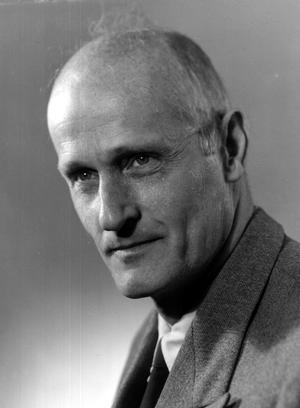
\includegraphics[width=\textwidth]{kleene.jpg}
%\end{column}
%\end{columns}
%
%\end{frame}

\begin{frame}{Regular Expressions over an Alphabet $\Sigma$}

A standard way to express languages for tokens.

\begin{enumerate}

\item $\epsilon$ is a regular expression that denotes $\{\epsilon\}$

\item If $a \in \Sigma$, $a$ is an RE that denotes $\{a\}$

\item If $r$ and $s$ denote languages $L(r)$ and $L(s)$,

\[
\begin{array}{lll}
(r)|(s) &\textsf{denotes}& L(r) \cup L(s) \\[10pt]
(r)(s) && \{ tu : t \in L(r), u \in L(s) \} \\[10pt]
(r)^* && \cup_{i=0}^{\infty} L(r)^i \\
& \textsf{where} & L(r)^0 = \{\epsilon\}\ \\
& \textsf{and} & L(r)^i = L(r) L(r)^{i-1} \\
\end{array}
\]

\end{enumerate}

\end{frame}

\begin{frame}{Regular Expression Examples}

$\Sigma = \{ a, b \}$

\begin{tabular}{ll}
\toprule
\textbf{Regexp.} & \textbf{Language} \\
\midrule
$a | b$ & $\{ a, b \}$ \\
$(a|b)(a|b)$ & $\{ aa, ab, ba, bb \}$ \\
$a^*$ & $\{ \epsilon, a, aa, aaa, aaaa, \ldots \}$ \\
$(a|b)^*$ & $\{ \epsilon, a, b, aa, ab, ba, bb, aaa, aab, aba, abb,
\ldots \}$ \\
$a | a^*b$ & $\{ a, b, ab, aab, aaab, aaaab, \ldots \}$ \\
\bottomrule
\end{tabular}

\end{frame}

\begin{frame}{Specifying Tokens with REs}

Typical choice: $\Sigma = $ ASCII characters, i.e., $\{
\texttt{\char`\ }, !, \texttt{"}, \#, \$, \ldots, \textrm{0},
\textrm{1}, \ldots, \textrm{9},
\ldots, \textrm{A}, \ldots, \textrm{Z}, \ldots, \texttt{\char`\~} \}$

\textbf{letters}: $\textrm{A} | \textrm{B} | \cdots | \textrm{Z} |
\textrm{a} | \cdots | \textrm{z}$

\textbf{digits}: $\textrm{0} | \textrm{1} | \cdots | \textrm{9}$

\textbf{identifier}: $\textbf{letter}\, (\, \textbf{letter}\, | \,
\textbf{digit}\, )^*$

\end{frame}

\begin{frame}{Implementing Scanners Automatically}

\begin{center}
\begin{tikzpicture}
  \matrix (re) [matrix of nodes,
    row sep=2pc,
    nodes={fill=white,draw,drop shadow}] {
    Regular Expressions (Rules) \\
    Nondeterministic Finite Automata \\
    Deterministic Finite Automata \\
    Tables \\
  };
\draw [->] (re-1-1) -- (re-2-1);
\draw [->] (re-2-1) -- node [right] {Subset Construction} (re-3-1);
\draw [->] (re-3-1) -- (re-4-1);
\end{tikzpicture}
\end{center}

\end{frame}

\begin{frame}[fragile]{Nondeterministic Finite Automata}

\begin{columns}
\begin{column}{0.4\textwidth}

``All strings containing an even number of 0's and 1's''

\vspace{2pc}

\begin{tikzpicture}
  \matrix [matrix of math nodes,
    nodes={circle,draw},
    column sep=2.5pc,
    row sep=2.5pc] {
    |[double] (A)| A & |(B)| B \\
    |(C)| C & |(D)| D \\
  };
  \begin{scope}[->, bend angle=15,bend left,inner sep=2pt]
    \draw (A) to node [above] {0} (B); 
    \draw (B) to node [below] {0} (A);
    \draw (B) to node [right] {1} (D); 
    \draw (D) to node [left]  {1} (B);
    \draw (D) to node [below] {0} (C); 
    \draw (C) to node [above] {0} (D);
    \draw (C) to node [left] {1} (A); 
    \draw (A) to node [right] {1} (C);
    \draw (A) ++ (-1.3pc,1pc) -- (A);
  \end{scope}
\end{tikzpicture}

\end{column}
\begin{column}{0.6\textwidth}

\begin{enumerate}\itemsep=0pt

\item Set of states $S:
\left\{
\begin{tikzpicture}[baseline=-4pt]
  \matrix [column sep=5pt,matrix of math nodes,nodes={circle,draw}] {
    |[double]| A & B & C & D \\ };
\end{tikzpicture}
\right\}$

\item Set of input symbols $\Sigma: \{ 0, 1 \}$

\item Transition function $\sigma : S \times \Sigma_{\epsilon} \rightarrow 2^S$

$\begin{array}{c|ccc}
\textbf{state} & \epsilon & 0 & 1 \\
\hline
A & \emptyset & \{B\} & \{C\} \\
B & \emptyset & \{A\} & \{D\} \\
C & \emptyset & \{D\} & \{A\} \\
D & \emptyset & \{C\} & \{B\} \\
\end{array}
$

\item Start state $s_0 :

\begin{tikzpicture}[baseline=-4pt]
  \node [draw,circle,double] {$A$};
\end{tikzpicture}
 $

\item Set of accepting states $F:
\left\{

\begin{tikzpicture}[baseline=-4pt]
  \node [draw,circle,double] {$A$};
\end{tikzpicture}
\right\}$

\end{enumerate}

\end{column}
\end{columns}

\end{frame}

\begin{frame}[fragile]{The Language induced by an NFA}

An NFA accepts an input string $x$ iff there is a path from the start
state to an accepting state that ``spells out'' $x$.

\vspace{2pc}

\begin{center}
\begin{tikzpicture}
  \matrix [matrix of math nodes,
    nodes={circle,draw},
    column sep=2.5pc,
    row sep=2.5pc] {
    |[double] (A)| A & |(B)| B \\
    |(C)| C & |(D)| D \\
  };
  \begin{scope}[->, bend angle=15,bend left,inner sep=2pt]
    \draw (A) to node [above] {0} (B); 
    \draw (B) to node [below] {0} (A);
    \draw (B) to node [right] {1} (D); 
    \draw (D) to node [left]  {1} (B);
    \draw (D) to node [below] {0} (C); 
    \draw (C) to node [above] {0} (D);
    \draw (C) to node [left] {1} (A); 
    \draw (A) to node [right] {1} (C);
    \draw (A) ++ (-1.3pc,1pc) -- (A);
  \end{scope}
\end{tikzpicture}
\end{center}

Show that the string ``010010'' is accepted.

\begin{tikzpicture}
  \matrix (z) [matrix of math nodes,
    nodes={circle,draw},
    column sep=1.5pc] {
    |[double]| A & B & D & C & D & B & |[double]| A \\
  };
  \begin{scope}[->,every node/.style={above}]
    \draw (z-1-1) -- node {0} (z-1-2);
    \draw (z-1-2) -- node {1} (z-1-3);
    \draw (z-1-3) -- node {0} (z-1-4);
    \draw (z-1-4) -- node {0} (z-1-5);
    \draw (z-1-5) -- node {1} (z-1-6);
    \draw (z-1-6) -- node {0} (z-1-7);
  \end{scope}
\end{tikzpicture}

\end{frame}

\begin{frame}[fragile]{Translating REs into NFAs (Thompson's algorithm)}

% http://hackingoff.com/compilers/regular-expression-to-nfa-dfa

\tikzset{every matrix/.style={matrix of math nodes,
                              nodes={circle,minimum size=1pc,draw}},
         initial text={},
         every state/.style={minimum size=1.5pc,fill=white},
         group/.style={ellipse,draw,fill=mBlue!30,minimum height=2.7pc, inner sep=-5pt},
         node distance=0.5pc and 2pc}

\begin{tabular}{ccc}
$a$ &
\begin{tikzpicture}[baseline=-4pt]
  \node[state,initial]              (A) {};
  \node[state,accepting,right=of A] (B) {};
  \path [->] (A) edge node [above] {$a$} (B);
\end{tikzpicture}
&
Symbol
\\[1pc]
$r_1 r_2$ &
\begin{tikzpicture}[baseline=-4pt]
  \node [state,initial]              (A) {};
  \node [state,right=of A]           (B) {};
  \node [state,accepting,right=of B] (C) {};
  \begin{pgfonlayer}{background}
    \node [group,fit=(A) (B)] {$r_1$};
    \node [group,fit=(B) (C)] {$r_2$};
  \end{pgfonlayer}
  \node [group,fill=none,fit=(A) (B)] {$r_1$};
\end{tikzpicture}
&
Sequence
\\[2pc]
$r_1 | r_2$ &
\begin{tikzpicture}[baseline=-4pt]
  \node [state,initial]              (A) {};
  \node [state,above right=of A]     (B) {};
  \node [state,right=of B]           (C) {};
  \node [state,accepting,below right=of C] (D) {};
  \node [state,below right=of A]     (E) {};
  \node [state,right=of E]     (F) {};
  \begin{pgfonlayer}{background}
    \node [group,fit=(B) (C)] {$r_1$};
    \node [group,fit=(E) (F)] {$r_2$};
  \end{pgfonlayer}
  \path [->] (A) edge node [above left] {$\epsilon$} (B)
             (A) edge node [below left] {$\epsilon$} (E)
             (C) edge node [above right] {$\epsilon$} (D)
             (F) edge node [below right] {$\epsilon$} (D);
\end{tikzpicture}
&
Choice
\\[3pc]
$(r)^*$ &
\begin{tikzpicture}[baseline=-4pt]
  \node [state,initial]              (A) {};
  \node [state,right=of A]           (B) {};
  \node [state,right=of B]           (C) {};
  \node [state,accepting,right=of C] (D) {};
  \begin{pgfonlayer}{background}
    \node [group,fit=(B) (C)] {$r$};
  \end{pgfonlayer}
  \path [->] (A) edge              node [above] {$\epsilon$} (B)
             (C) edge              node [above] {$\epsilon$} (D)
             (C) edge [bend right=80] node [above] {$\epsilon$} (B)
             (A) edge [bend right=40] node [below] {$\epsilon$} (D);
\end{tikzpicture}
&
Kleene Closure
 \\
\end{tabular}

\end{frame}

\begin{frame}[fragile]{Why So Many Extra States and Transitions?}

Invariant: Single start state; single end state; at most two outgoing
arcs from any state: helpful for simulation.

What if we used this simpler rule for Kleene Closure?

\tikzset{every matrix/.style={matrix of math nodes,
                              nodes={circle,minimum size=1pc,draw}},
         initial text={},
         every state/.style={minimum size=1.5pc,fill=white},
         group/.style={ellipse,draw,fill=mBlue!30,minimum height=2.7pc, inner sep=-5pt},
         node distance=0.5pc and 2pc}

\begin{tikzpicture}[baseline=-4pt]
  \node [state,initial]              (A) {};
  \node [state,accepting,right=of A] (B) {};
  \begin{pgfonlayer}{background}
    \node [group,fit=(A) (B)] {$r$};
  \end{pgfonlayer}
  \path [->] (B) edge [bend right=80] node [above] {$\epsilon$} (A)
             (A) edge [bend right=80] node [below] {$\epsilon$} (B);
\end{tikzpicture}

Now consider $a^*b^*$ with this rule:

\begin{tikzpicture}[baseline=-4pt]
\node [state,initial] (A) {};
\node [state,right=of A] (B) {};
\node [state,accepting,right=of B] (C) {};
  \path [->] (A) edge                 node [above] {$a$}        (B)
             (B) edge                 node [above] {$b$}        (C)
             (B) edge [bend right=80] node [above] {$\epsilon$} (A)
             (A) edge [bend right=80] node [below] {$\epsilon$} (B)
             (C) edge [bend right=80] node [above] {$\epsilon$} (B)
             (B) edge [bend right=80] node [below] {$\epsilon$} (C);
\end{tikzpicture}

Is this right?

\end{frame}

\def\aabb#1#2#3#4#5#6#7#8#9{
  \begin{tikzpicture}[node distance=0.7pc and 1pc,                      
                      every state/.style={inner sep=1pt,
                        fill=white,
                        minimum size=14pt},
                        initial text={}]
    \node [state,fill=\filled#1,initial] (0) {0};
    \node [state,fill=\filled#2,right=of 0] (1) {1};
    \node [state,fill=\filled#3,above right=of 1] (2) {2};
    \node [state,fill=\filled#4,right=of 2] (3) {3};
    \node [state,fill=\filled#5,below right=of 1] (4) {4};
    \node [state,fill=\filled#6,right=of 4] (5) {5};
    \node [state,fill=\filled#7,below right=of 3] (6) {6};
    \node [state,fill=\filled#8,right=of 6] (7) {7};
    \node [state,fill=\filled#9,right=of 7] (8) {8};
\aabbtwo
}

\def\aabbtwo#1#2{
    \node [state,fill=\filled#1,right=of 8] (9) {9};
    \node [state,fill=\filled#2,accepting,right=of 9] (10) {10};
    \path [->] (0) edge node [above] {$\epsilon$} (1)
               (1) edge node [above left] {$\epsilon$} (2)
               (2) edge node [above] {$a$} (3)
               (1) edge node [below left] {$\epsilon$} (4)
               (4) edge node [below] {$b$} (5)            
               (3) edge node [above right] {$\epsilon$} (6)
               (5) edge node [below right] {$\epsilon$} (6)
               (6) edge node [above] {$\epsilon$} (7)
               (7) edge node [above] {$a$} (8)
               (8) edge node [above] {$b$} (9)
               (9) edge node [above] {$b$} (10)
               (6) edge [bend right=90,looseness=1.5] node [above] {$\epsilon$} (1)
               (0) edge [bend right=70] node [below] {$\epsilon$} (7)
            ;
  \end{tikzpicture}
}

\begin{frame}[fragile]{Translating REs into NFAs}

Example: Translate $(a|b)^*abb$ into an NFA. Answer:

\aabb00000000000

Show that the string ``$aabb$'' is accepted. Answer:

\begin{tikzpicture}[node distance=1pc,every state/.style={inner sep=1pt,minimum size=14pt},
    initial text={}]
  \node [state,initial] (0) {0};
  \node [state,right=of 0] (1) {1};
  \node [state,right=of 1] (2) {2};
  \node [state,right=of 2] (3) {3};
  \node [state,right=of 3] (6) {6};
  \node [state,right=of 6] (7) {7};
  \node [state,right=of 7] (8) {8};
  \node [state,right=of 8] (9) {9};
  \node [state,right=of 9,accepting] (10) {10};
  \path [->] (0) edge node [above] {$\epsilon$} (1)
             (1) edge node [above] {$\epsilon$} (2)
             (2) edge node [above] {$a$} (3)
             (3) edge node [above] {$\epsilon$} (6)
             (6) edge node [above] {$\epsilon$} (7)
             (7) edge node [above] {$a$} (8)
             (8) edge node [above] {$b$} (9)
             (9) edge node [above] {$b$} (10)
  ;
\end{tikzpicture}


\end{frame}

\begin{frame}{Simulating NFAs}

Problem: you must follow the ``\alert{right}'' arcs to show that a string is
accepted.  How do you know which arc is right?

Solution: follow them all and sort it out later.

``Two-stack'' NFA simulation algorithm:

\begin{enumerate}
\item Initial states: the $\epsilon$-closure of the start state
\item For each character $c$,
\begin{itemize}
\item New states: follow all transitions labeled $c$
\item Form the $\epsilon$-closure of the current states
\end{itemize}
\item Accept if any final state is accepting
\end{enumerate}

\end{frame}

\def\step#1#2{
\begin{frame}{Simulating an NFA: #2}
\aabb #1
\end{frame}
}
\def\point{\mathord{\cdot}}
%     01234 567890
\step{10000 000000}{$\point aabb$, Start}
\step{11101 001000}{$\point aabb$, $\epsilon$-closure}
\step{00010 000100}{$a\point abb$}
\step{01111 011100}{$a\point abb$, $\epsilon$-closure}
\step{00010 000100}{$aa\point bb$}
\step{01111 011100}{$aa\point bb$, $\epsilon$-closure}
\step{00000 100010}{$aab\point b$}
\step{01101 111010}{$aab\point b$, $\epsilon$-closure}
\step{00000 100001}{$aabb\point $}
\step{01101 111001}{$aabb\point$, Done}

\begin{frame}{Deterministic Finite Automata}

Restricted form of NFAs:

\begin{itemize}
\item No state has a transition on $\epsilon$
\item For each state $s$ and symbol $a$, there is at most one edge
  labeled $a$ leaving $s$.
\end{itemize}

Differs subtly from the definition used in COMS W3261 (Sipser,
\emph{Introduction to the Theory of Computation})

Very easy to check acceptance: simulate by maintaining current state.
Accept if you end up on an accepting state. Reject if you end on a
non-accepting state or if there is no transition from the current
state for the next symbol.

\end{frame}

\begin{frame}[fragile]{Deterministic Finite Automata}

\begin{ocamllex}
{
   type token = ELSE | ELSEIF
}

rule token =
  parse "else"   { ELSE }
      | "elseif" { ELSEIF }
\end{ocamllex}

\begin{tikzpicture}[node distance=1.5pc,
    every state/.style={inner sep=1pt,minimum size=14pt},
    initial text={}]
  \node [state,initial] (0) {};
  \node [state,right=of 0] (1) {};
  \node [state,right=of 1] (2) {};
  \node [state,right=of 2] (3) {};
  \node [state,right=of 3,accepting] (4) {};
  \node [state,right=of 4] (5) {};
  \node [state,right=of 5,accepting] (6) {};
  \path [->] (0) edge node [above] {e} (1)
             (1) edge node [above] {l} (2)
             (2) edge node [above] {s} (3)
             (3) edge node [above] {e} (4)
             (4) edge node [above] {i} (5)
             (5) edge node [above] {f} (6);
\end{tikzpicture}

\end{frame}


\begin{frame}[fragile]{Deterministic Finite Automata}

\begin{ocamllex}
{ type token = IF | ID of string | NUM of string }

rule token =
  parse "if"                                { IF }
      | ['a'-'z'] ['a'-'z' '0'-'9']* as lit { ID(lit) }
      | ['0'-'9']+                   as num { NUM(num) }
\end{ocamllex}

\begin{tikzpicture}[node distance=3pc and 5pc,
    every state/.style={inner sep=1pt,minimum size=30pt},
    initial text={}]
  \node [state,initial] (start) {};
  \node [state,below right=of start,accepting] (num) {NUM};
  \node [state,above right=of start,accepting] (id1) {ID};
  \node [state,right=of id1,accepting] (if) {IF};
  \node [state,below=of if,accepting] (id2) {ID};
  \path [->] (start) edge node [below left] {0--9} (num)
             (start) edge node [above] {i} (id1)
             (start) edge node [above] {a--hj--z} (id2)
             (id1) edge node [above] {f} (if)
             (if) edge node [right] {a--z0--9} (id2)
             (id1) edge node [above,sloped] {a--eg--z0--9} (id2)
             (num) edge [loop right] node [right] {0--9} ()
             (id2) edge [loop right] node [right] {a--z0--9} ();
\end{tikzpicture}

\end{frame}

\begin{frame}{Building a DFA from an NFA}

Subset construction algorithm

Simulate the NFA for all possible inputs and track the states that
appear.

Each unique state during simulation becomes a state in the DFA.

\end{frame}

\def\aabbz#1#2#3#4#5#6#7#8#9{
\begin{scope}[node distance=3pt and 2pt,
                      every state/.style={inner sep=1pt,
                        fill=white,
                        minimum size=5pt}]
    \node [state,fill=\filled#2] at ($(#1)+(left:1)$) (0) {};
    \node [state,fill=\filled#3,right=of 0] (1) {};
    \node [state,fill=\filled#4,above right=of 1] (2) {};
    \node [state,fill=\filled#5,right=of 2] (3) {};
    \node [state,fill=\filled#6,below right=of 1] (4) {};
    \node [state,fill=\filled#7,right=of 4] (5) {};
    \node [state,fill=\filled#8,below right=of 3] (6) {};
    \node [state,fill=\filled#9,right=of 6] (7) {};
\aabbztwo
}

\def\aabbztwo#1#2#3{
    \node [state,fill=\filled#1,right=of 7] (8) {};
    \node [state,fill=\filled#2,right=of 8] (9) {};
    \node [state,fill=\filled#3,accepting,right=of 9] (10) {};
    \path (0) edge node [above] {} (1)
          (1) edge node [above left] {} (2)
          (2) edge node [above] {} (3)
          (1) edge node [below left] {} (4)
          (4) edge node [below] {} (5)            
          (3) edge node [above right] {} (6)
          (5) edge node [below right] {} (6)
          (6) edge node [above] {} (7)
          (7) edge node [above] {} (8)
          (8) edge node [above] {} (9)
          (9) edge node [above] {} (10)
          (6) edge [bend right=90,looseness=2.5] node [above] {} (1)
          (0) edge [bend right=80,looseness=1.5] node [below] {} (7)
            ;
\end{scope}
}

%                  01234567890
\def\sa#1{\aabbz{#1}11101001000}
\def\sb#1{\aabbz{#1}01111011100}
\def\sc#1{\aabbz{#1}01101111000}
\def\sd#1{\aabbz{#1}01101111010}
\def\se#1{\aabbz{#1}01101111001}

% sa -a-> sb -a-> sb -b-> sd -b-> se
% sa -b-> sc -b-> sc -a-> sb
% sd -a-> sb
% se -a-> sb
% se -b-> sc

\begin{frame}[t]{Subset construction for $(a|b)^*abb$}
  \begin{tikzpicture}[nfastate/.style={state,inner sep=25pt,fill=mBlue!30},
    initial text={}]
    \node [initial,nfastate] (a) {};
    \sa{a}
    \pause
    \node [nfastate,right=of a] (b) {}; % \sb \\ };
    \sb{b}
    \node [nfastate,below=of a,xshift=4pc] (c) {}; % \sc \\ };
    \sc{c}
    \path [->] (a) edge node [above] {a} (b)
               (a) edge node [left] {b} (c);
    \pause
    \node [nfastate,right=of b] (d) {};% \sd \\ };
    \sd{d}
    \path [->,every loop/.style={looseness=3}]
               (b) edge [loop above] node [above] {a} ()
               (b) edge [bend left=20] node [above] {b} (d)
               (c) edge [loop left] node [left] {b} ()
               (c) edge node [below right] {a} (b);
    \pause
    \node [nfastate,accepting,right=of c] (e) {};% \se \\ };
    \se{e}
    \path [->]
          (d) edge [bend left=20] node[below] {a} (b)
          (d) edge node [right] {b} (e);
    \pause
    \path [->]
          (e) edge node [below left] {a} (b)
          (e) edge node [below] {b} (c);
  \end{tikzpicture}
\end{frame}

\begin{frame}[t]{Result of subset construction for $(a|b)^*abb$}
\begin{center}
  \begin{tikzpicture}[node distance=4pc,initial text={}]
    \node [initial,state] (a) {};
    \node [state,right=of a] (b) {};
    \node [state,below=of a,xshift=3pc] (c) {};
    \path [->] (a) edge node [above] {a} (b)
               (a) edge node [left] {b} (c);
    \node [state,right=of b] (d) {};
    \path [->,every loop/.style={looseness=3}]
               (b) edge [loop above] node [above] {a} ()
               (b) edge [bend left=20] node [above] {b} (d)
               (c) edge [loop left] node [left] {b} ()
               (c) edge node [below right] {a} (b);
    \node [state,accepting,right=of c] (e) {};
    \path [->]
          (d) edge [bend left=20] node[below] {a} (b)
          (d) edge node [right] {b} (e);
    \path [->]
          (e) edge node [below left] {a} (b)
          (e) edge node [below] {b} (c);
  \end{tikzpicture}

\emph{Is this minimal?}
\end{center}
\end{frame}


\begin{frame}[t]{Minimized result for $(a|b)^*abb$}
\begin{center}
  \begin{tikzpicture}[node distance=4pc,initial text={}]
    \node [initial,state] (a) {};
    \node [state,right=of a] (b) {};
    \path [->] (a) edge node [above] {a} (b);
    \node [state,right=of b] (d) {};
    \path [->,every loop/.style={looseness=3}]
               (b) edge [loop above] node [above] {a} ()
               (b) edge [bend left=20] node [above] {b} (d)
               (a) edge [loop above] node [above] {b} ();
    \node [state,accepting,below=of b] (e) {};
    \path [->]
          (d) edge [bend left=20] node[below] {a} (b)
          (d) edge node [right] {b} (e);
    \path [->]
          (e) edge node [below left] {a} (b)
          (e) edge node [below] {b} (a);
  \end{tikzpicture}

\end{center}
\end{frame}

\begin{frame}[fragile]{Transition Table Used In the Dragon Book}

Problem: Translate $(a|b)^*abb$ into an NFA and perform subset
construction to produce a DFA.

Solution:

\vspace{-2pc}

\aabb00000000000

\begin{columns}
\begin{column}{0.6\textwidth}
\begin{tabular}{lccc}
\toprule
\textbf{NFA State} & \textbf{DFA State} & \textbf{a} & \textbf{b} \\
\midrule
\{0,1,2,4,7\} & A & B & C \\
\{1,2,3,4,6,7,8\} & B & B & D \\
\{1,2,4,5,6,7\} & C & B & C \\
\{1,2,4,5,6,7,9\} & D & B & E \\
\{1,2,4,5,6,7,10\} & E & B & C \\
\bottomrule
\end{tabular}
\end{column}
\begin{column}{0.4\textwidth}
  \begin{tikzpicture}[node distance=2pc,initial text={},
                      every state/.style={inner sep=1pt,minimum size=10pt}]
    \node [initial,state] (a) {A};
    \node [state,right=of a] (b) {B};
    \node [state,below=of a,xshift=1.5pc] (c) {C};
    \path [->] (a) edge node [above] {a} (b)
               (a) edge node [left] {b} (c);
    \node [state,right=of b] (d) {D};
    \path [->,every loop/.style={looseness=3}]
               (b) edge [loop above] node [above] {a} ()
               (b) edge [bend left=20] node [above] {b} (d)
               (c) edge [loop left] node [left] {b} ()
               (c) edge node [above left] {a} (b);
    \node [state,accepting,right=of c] (e) {E};
    \path [->]
          (d) edge [bend left=20] node[below] {a} (b)
          (d) edge node [right] {b} (e);
    \path [->]
          (e) edge node [below left] {a} (b)
          (e) edge node [below] {b} (c);
  \end{tikzpicture}
\end{column}
\end{columns}
\end{frame}


\begin{frame}{Subset Construction}

An DFA can be exponentially larger than the corresponding NFA.

$n$ states versus $2^n$

Tools often try to strike a balance between the two representations.

\end{frame}

\part{Lexical Analysis with Ocamllex}

\begin{frame}[fragile]{Constructing Scanners with Ocamllex}

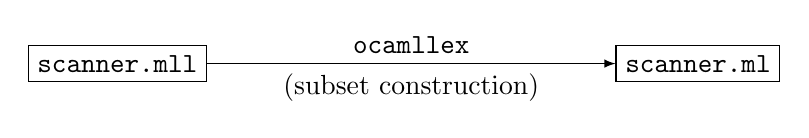
\begin{tikzpicture}
  \node [draw] (mll) {\texttt{scanner.mll}};
  \node [draw,right=15pc] (ml) {\texttt{scanner.ml}};
  \draw [->] (mll) -- node [above] {\texttt{ocamllex}}
                      node [below] {(subset construction)} (ml);
\end{tikzpicture}

An example:

\medskip

scanner.mll

\vspace{4pt}

\begin{ocamllex}
{ open Parser }

rule token =
  parse [' ' '\t' '\r' '\n'] { token lexbuf }
      | '+'                  { PLUS }
      | '-'                  { MINUS }
      | '*'                  { TIMES }
      | '/'                  { DIVIDE }
      | ['0'-'9']+ as lit    { LITERAL(int_of_string lit) }
      | eof                  { EOF }
\end{ocamllex}

\end{frame}

\begin{frame}[fragile]{Ocamllex Specifications}

\begin{ocamllex}
{
  (* Header: verbatim OCaml code; mandatory *)
}

(* Definitions: optional *)
let ident = regexp
let ...

(* Rules: mandatory *)
rule entrypoint1 [arg1 ... argn] =
  parse pattern1 { action (* OCaml code *) }
      | ...
      | patternn { action }
and entrypoint2 [arg1 ... argn]} =
  ...
and ...

{
  (* Trailer: verbatim OCaml code; optional *)
}
\end{ocamllex}

\end{frame}

\begin{frame}[fragile]{Patterns (In Order of Decreasing Precedence)}
\footnotesize
\begin{tabular}{ll}
\toprule
\textbf{Pattern} & \textbf{Meaning} \\
\midrule
\verb|'c'| & A single character\\
\verb|_| & Any character (underline)\\
\verb|eof| & The end-of-file\\
\verb|"foo"| & A literal string\\
\verb|['1' '5' 'a'-'z']| & ``1,'' ``5,'' or any lowercase letter\\
\verb|[^ '0'-'9']| & Any character except a digit \\
\verb|(| \emph{pattern} \verb|)| & Grouping\\
\emph{identifier} & A pattern defined in the \texttt{let} section\\
\midrule
\emph{pattern} \verb|*| & Zero or more \emph{pattern}s\\
\emph{pattern} \verb|+| & One or more \emph{pattern}s\\
\midrule
\emph{pattern} \verb|?| & Zero or one \emph{pattern}s\\
\midrule
\emph{pattern}$_1$ \emph{pattern}$_2$  & \emph{pattern}$_1$ followed by \emph{pattern}$_2$\\
\midrule
\emph{pattern}$_1$ \verb+|+ \emph{pattern}$_2$  & Either \emph{pattern}$_1$ or \emph{pattern}$_2$\\
\midrule
\emph{pattern} \verb|as| \emph{id}  & Bind the matched pattern to variable \emph{id}\\
\bottomrule
\end{tabular}

\end{frame}

\begin{frame}[fragile]{An Example}
\small
\begin{ocamllex}
{ type token = PLUS | IF | ID of string | NUM of int }

let letter = ['a'-'z' 'A'-'Z']
let digit = ['0'-'9']

rule token =
 parse [' ' '\n' '\t'] { token lexbuf } (* Ignore whitespace *)

     | '+' { PLUS }                     (* A symbol *)

     | "if" { IF }                      (* A keyword *)
                                        (* Identifiers *)
     | letter (letter | digit | '_')* as id { ID(id) }
                                        (* Numeric literals *)
     | digit+ as lit { NUM(int_of_string lit) }

     | "/*" { comment lexbuf }          (* C-style comments *)

and comment =
  parse "*/" { token lexbuf } (* Return to normal scanning *)
      | _ { comment lexbuf }  (* Ignore other characters *)
\end{ocamllex}

\end{frame}

\begin{frame}{Free-Format Languages}
Typical style arising from scanner/parser division

Program text is a series of tokens possibly separated by whitespace
and comments, which are both ignored.

\begin{itemize}
\item keywords (\texttt{if while})
\item punctuation (\texttt{, ( +})
\item identifiers (\texttt{foo bar})
\item numbers (\texttt{10 -3.14159e+32})
\item strings (\texttt{"A String"})
\end{itemize}

\end{frame}

\begin{frame}{Free-Format Languages}

Java \hfil C \hfil C++ \hfil C\# \hfil Algol \hfil Pascal

Some deviate a little (e.g., C and C++ have a separate preprocessor)

But not all languages are free-format.
\end{frame}

%\begin{frame}[fragile]{FORTRAN 77}
%
%FORTRAN 77 is not free-format.  72-character lines:
%
%\begin{fortran}
%100   IF(IN .EQ. 'Y' .OR. IN .EQ. 'y' .OR.
%     $   IN .EQ. 'T' .OR. IN .EQ. 't') THEN
%\end{fortran}
%
%% $
%
%{
%\[\underbrace{\framebox{\textrm{1}} \cdots \framebox{\textrm{5}}}_{\mbox{Statement label}}
%\underbrace{\framebox{\textrm{6}}}_{\mbox{Continuation}}
%\underbrace{\framebox{\textrm{7}} \cdots \framebox{\textrm{72}}}_{\mbox{Normal}}\]
%}
%
%When column 6 is not a space, line is considered part of the
%previous.
%
%Fixed-length line works well with a one-line buffer.
%
%Makes sense on punch cards. 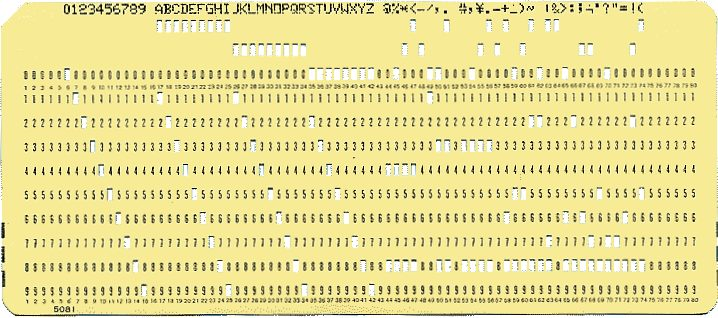
\includegraphics[width=8pc]{punchcard.jpg}
%
%\end{frame}

\begin{frame}[fragile]{Python}

The Python scripting language groups with indentation

\begin{python}
i = 0
while i < 10:
    i = i + 1
    print i    # Prints 1, 2, ..., 10

i = 0
while i < 10:
    i = i + 1
print i        # Just prints 10
\end{python}

This is succinct, but can be error-prone.

How do you wrap a conditional around instructions?

\end{frame}

\begin{frame}[fragile]{Syntax and Language Design}

Does syntax matter?  Yes and no

More important is a language's \emph{semantics}---its meaning.

The syntax is aesthetic, but can be a religious issue.

But aesthetics matter to people, and can be critical.

Verbosity does matter: smaller is usually better.

Too small can be problematic: APL is a succinct language with its
own character set.

There are no APL programs, only puzzles.

\end{frame}

\begin{frame}[fragile]{Syntax and Language Design}

Some syntax is error-prone.  Classic \textsc{fortran} example:

\begin{fortran}
DO 5 I = 1,25  ! Loop header (for i = 1 to 25)
DO 5 I = 1.25  ! Assignment to variable DO5I
\end{fortran}

Trying too hard to reuse existing syntax in C++:

\begin{cpp}
vector< vector<int> > foo;
vector<vector<int>> foo; // Syntax error
\end{cpp}

C distinguishes \verb|>| and \verb|>>| as different operators.

Bjarne Stroustrup tells me they have finally fixed this.

\end{frame}

\part{Modeling Sentences}

\begin{frame}{Simple Sentences Are Easy to Model}

The boy eats hot dogs.

The dog eats ice cream.

Every happy girl eats candy.

A dog eats candy.

The happy happy dog eats hot dogs.

\begin{tikzpicture}[node distance=0.5pc and 2pc]
  \node [text width=2.5pc] (s1) {The \break A \break Every};
  \node [above right=of s1] (s2) {happy};
  \node [text width=2pc,below right=of s2] (s3) {boy\break girl\break dog};
  \node [right=of s3] (s4) {eats};
  \node [text width=4pc,right=of s4] (s5) {hot dogs.\break ice cream.\break candy.};
  \path [->]
    (s1) edge (s2)
    (s2) edge [loop above] ()
    (s2) edge (s3)
    (s1) edge (s3)
    (s3) edge (s4)
    (s4) edge (s5)
  ;
\end{tikzpicture}

\tiny Pinker, \emph{The Language Instinct}

\end{frame}

\begin{frame}{Richer Sentences Are Harder}

  If the boy eats hot dogs, then the girl eats ice cream.

  Either the boy eats candy, or every dog eats candy.


\begin{tikzpicture}[node distance=0.5pc and 1pc]
  \node [text width=2pc] (s0) {Either\break If};
  \node [text width=2.5pc,right=of s0] (s1) {the \break a \break every};
  \node [above right=of s1] (s2) {happy};
  \node [text width=1.8pc,below right=of s2] (s3) {boy\break girl\break dog};
  \node [right=of s3] (s4) {eats};
  \node [text width=4pc,right=of s4] (s5) {hot dogs\break ice cream\break candy};
  \node [text width=2pc,right=of s5] (s6) {or\break then};
  \path [->]
    (s0) edge (s1)
    (s1) edge (s2)
    (s2) edge [loop above] ()
    (s2) edge (s3)
    (s1) edge (s3)
    (s3) edge (s4)
    (s4) edge (s5)
    (s5) edge (s6)
    (s6) edge [bend left=80,looseness=0.4] (s1);
  ;
\end{tikzpicture}

\centerline{\emph{Does this work?}}

\end{frame}

\begin{frame}{Automata Have Poor Memories}

Want to ``remember'' whether it is an ``either-or'' or ``if-then''
sentence.  Only solution: duplicate states.

\tiny

\begin{tikzpicture}[node distance=0.3pc and 0.5pc]
  \node (s0) {};
  \node at (1pc,2pc) (sa0) {Either};
  \node [text width=1.5pc,right=of sa0] (sa1) {the \break a \break every};
  \node [above right=of sa1] (sa2) {happy};
  \node [text width=1.2pc,below right=of sa2] (sa3) {boy\break girl\break dog};
  \node [right=of sa3] (sa4) {eats};
  \node [text width=2.5pc,right=of sa4] (sa5) {hot dogs\break ice cream\break candy};
  \node [right=of sa5] (sa6) {or};
  \path [->]
    (sa0) edge (sa1)
    (sa1) edge (sa2)
    (sa2) edge [loop above] ()
    (sa2) edge (sa3)
    (sa1) edge (sa3)
    (sa3) edge (sa4)
    (sa4) edge (sa5)
    (sa5) edge (sa6);

  \node at (1pc,-2pc) (sb0) {If};
  \node [text width=1.5pc,right=of sb0] (sb1) {the \break a \break every};
  \node [above right=of sb1] (sb2) {happy};
  \node [text width=1.2pc,below right=of sb2] (sb3) {boy\break girl\break dog};
  \node [right=of sb3] (sb4) {eats};
  \node [text width=2.5pc,right=of sb4] (sb5) {hot dogs\break ice cream\break candy};
  \node [right=of sb5] (sb6) {then};
  \path [->]
    (s0) edge (sa0)
    (s0) edge (sb0)
    (sb0) edge (sb1)
    (sb1) edge (sb2)
    (sb2) edge [loop above] ()
    (sb2) edge (sb3)
    (sb1) edge (sb3)
    (sb3) edge (sb4)
    (sb4) edge (sb5)
    (sb5) edge (sb6);

  \node [text width=1.5pc] at (16pc,0pc) (sc1) {the \break a \break every};
  \node [above right=of sc1] (sc2) {happy};
  \node [text width=1.2pc,below right=of sc2] (sc3) {boy\break girl\break dog};
  \node [right=of sc3] (sc4) {eats};
  \node [text width=2.5pc,right=of sc4] (sc5) {hot dogs\break ice cream\break candy};
  \path [->]
    (sa6) edge (sc1)
    (sb6) edge (sc1)
    (sc1) edge (sc2)
    (sc2) edge [loop above] ()
    (sc2) edge (sc3)
    (sc1) edge (sc3)
    (sc3) edge (sc4)
    (sc4) edge (sc5);

\end{tikzpicture}

\end{frame}

\def\s#1{\hfil$#1:$\hfil\break}
\begin{frame}{Automata in the form of Production Rules}

Problem: automata do not remember where they've been

{\footnotesize\ttfamily
\begin{tabular}{l}
$S \rightarrow$ Either    $A$ \\
$S \rightarrow$ If        $A$ \\
$A \rightarrow$ the       $B$ \\
$A \rightarrow$ the       $C$ \\
$A \rightarrow$ a         $B$ \\
$A \rightarrow$ a         $C$ \\
$A \rightarrow$ every     $B$ \\
$A \rightarrow$ every     $C$ \\
$B \rightarrow$ happy     $B$ \\
$B \rightarrow$ happy     $C$ \\
$C \rightarrow$ boy       $D$ \\
$C \rightarrow$ girl      $D$ \\
$C \rightarrow$ dog       $D$ \\
$D \rightarrow$ eats      $E$ \\
$E \rightarrow$ hot dogs  $F$ \\
$E \rightarrow$ ice cream $F$ \\
$E \rightarrow$ candy     $F$ \\
$F \rightarrow$ or        $A$ \\
$F \rightarrow$ then      $A$ \\
$F \rightarrow$ $\epsilon$ \\
\end{tabular}}
\tiny
\begin{tikzpicture}[node distance=0.3pc and 0.5pc,
  every node/.style={draw}]
  \node [text width=1.5pc] (s0) {\s S Either\break If};
  \node [text width=1.5pc,right=of s0] (s1) {\s A the \break a \break every};
  \node [above right=of s1] (s2) {\s B happy};
  \node [text width=1.2pc,below right=of s2] (s3) {\s C boy\break girl\break dog};
  \node [right=of s3] (s4) {\s D eats};
  \node [text width=2.5pc,right=of s4] (s5) {\s E hot dogs\break ice cream\break candy};
  \node [text width=1.5pc,right=of s5] (s6) {\s F or\break then};
  \path [->]
    (s0) edge (s1)
    (s1) edge (s2)
    (s2) edge [loop above] ()
    (s2) edge (s3)
    (s1) edge (s3)
    (s3) edge (s4)
    (s4) edge (s5)
    (s5) edge (s6)
    (s6) edge [bend left=80,looseness=0.4] (s1);
  ;
\end{tikzpicture}

\end{frame}

\begin{frame}{Solution: Context-Free Grammars}

Context-Free Grammars have the ability to ``call subroutines:''

{\ttfamily
\begin{tabular}{ll}
$S \rightarrow$ Either $P$, or $P$. & \rmfamily \alert{Exactly two $P$s}\\
$S \rightarrow$ If $P$, then $P$. \\
$P \rightarrow$ $A$ $H$ $N$ eats $O$ & \rmfamily \alert{One each of $A$, $H$, $N$, and
    $O$} \\
$A \rightarrow$ the \\
$A \rightarrow$ a \\
$A \rightarrow$ every \\
$H \rightarrow$ happy $H$ & \rmfamily \alert{$H$ is ``happy'' zero or more times} \\
$H \rightarrow$ $\epsilon$ \\
$N \rightarrow$ boy \\
$N \rightarrow$ girl \\
$N \rightarrow$ dog \\
$O \rightarrow$ hot dogs \\
$O \rightarrow$ ice cream \\
$O \rightarrow$ candy \\
\end{tabular}
}

\end{frame}

\def\tok#1{\textbf{\texttt{#1}}}

\begin{frame}{A Context-Free Grammar for a Simplified C}
\small
\[
\begin{array}{r@{\hspace{3pt}}c@{\hspace{3pt}}l}
\textit{program} & \rightarrow & \epsilon |
   \textit{program}\ \textit{vdecl} |
   \textit{program}\ \textit{fdecl} \\[5pt]
\textit{fdecl} & \rightarrow &
\tok{id}\ \tok{(}\ \textit{formals}\ \tok{)}\ \tok{\{}\ \textit{vdecls}\ \textit{stmts}\ \tok{\}}
\\[5pt]
\textit{formals} & \rightarrow & \tok{id} |
\textit{formals}\ \tok{,}\ \tok{id} \\[5pt]
\textit{vdecls} & \rightarrow & \textit{vdecl} | \textit{vdecls}\ \textit{vdecl} \\[5pt]
\textit{vdecl} & \rightarrow & \tok{int}\ \tok{id}\ \tok{;} \\[5pt]
\textit{stmts} & \rightarrow & \epsilon | \textit{stmts}\ \textit{stmt} \\[5pt]
\textit{stmt} & \rightarrow & \textit{expr}\ \tok{;} |
\tok{return}\ \textit{expr}\ \tok{;} |
\tok{\{}\ \textit{stmts}\ \tok{\}} |
\tok{if}\ \tok{(}\ \textit{expr}\ \tok{)}\ \textit{stmt} | \\&&
\tok{if}\ \tok{(}\ \textit{expr}\ \tok{)}\ \textit{stmt}\ \tok{else}\ \textit{stmt}
| \\&&
\tok{for}\ \tok{(}\ \textit{expr}\ \tok{;}\ \textit{expr}\ \tok{;}\ \textit{expr}\ \tok{)}\ \textit{stmt}
|
\tok{while}\ \tok{(}\ \textit{expr}\ \tok{)}\ \textit{stmt}
\\[5pt]
\textit{expr} & \rightarrow &
\tok{lit} | \tok{id} |
\tok{id}\ \tok{(}\ \textit{actuals}\ \tok{)} |
\tok{(}\ \textit{expr}\ \tok{)} | \\&&
\textit{expr}\ \tok{+}\ \textit{expr} |
\textit{expr}\ \tok{-}\ \textit{expr} |
\textit{expr}\ \tok{*}\ \textit{expr} |
\textit{expr}\ \tok{/}\ \textit{expr} | \\&&
\textit{expr}\ \tok{==}\ \textit{expr} |
\textit{expr}\ \tok{!=}\ \textit{expr} |
\textit{expr}\ \tok{<}\ \textit{expr} |
\textit{expr}\ \tok{<=}\ \textit{expr} |  \\&&
\textit{expr}\ \tok{>}\ \textit{expr} |
\textit{expr}\ \tok{>=}\ \textit{expr} |
\textit{expr}\ \tok{=}\ \textit{expr}
\\[5pt]
\textit{actuals} & \rightarrow & \textit{expr} | \textit{actuals}
\tok{,} \textit{expr} \\
\end{array}
\]

\end{frame}

\part{Constructing Grammars and Ocamlyacc}
%\frame{\partpage}

\begin{frame}{Parsing}
Objective: build an abstract syntax tree (AST) for the token sequence
from the scanner.

\begin{center}
\texttt{2 * 3 + 4} \hspace{3pc} $\Rightarrow$ \hspace{3pc}
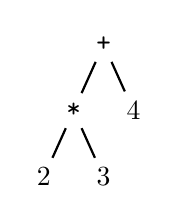
\begin{tikzpicture}[parsetree]
  \path \plus{\mult{\lit2}{\lit3}}{\lit4};
\end{tikzpicture}
\end{center}

\medskip

Goal: verify the syntax of the program, discard irrelevant
information, and ``understand'' the structure of the program.

Parentheses and most other forms of punctuation removed.

\end{frame}

\begin{frame}{Ambiguity}

\centerline{\emph{One morning I shot an elephant in my pajamas.}}

\pause

\centerline{\emph{How he got in my pajamas I don't know. ---Groucho Marx}}

\vfill

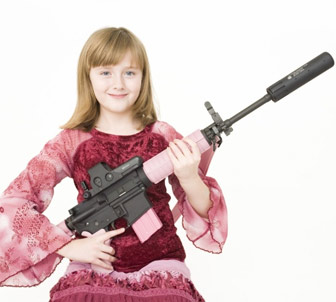
\includegraphics[height=0.4\textheight]{guns_girl.jpg} \hfill
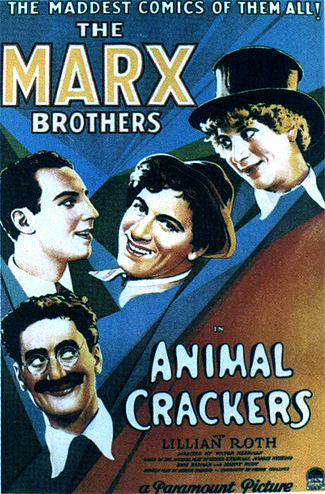
\includegraphics[height=0.4\textheight]{AnimalCrackers.jpg} \hfill

\includegraphics[height=0.4\textheight]{elephant-in-pajamas.jpg}

\end{frame}

\begin{frame}{Ambiguity in English}

\centerline{\emph{I shot an elephant in my pajamas}}

\begin{minipage}{0.35\textwidth}
\footnotesize
\begin{tabular}{@{}>{\itshape}l>{$}c<{$}>{\itshape}l@{}}
S & \rightarrow & NP VP \\
VP & \rightarrow & V NP \\
VP & \rightarrow & V NP PP \\
NP & \rightarrow & NP PP \\
NP & \rightarrow & Pro \\
NP & \rightarrow & Det Noun \\
NP & \rightarrow & Poss Noun \\
PP & \rightarrow & P NP \\
V & \rightarrow & \upshape shot \\
Noun & \rightarrow & \upshape elephant \\
Noun & \rightarrow & \upshape pajamas \\
Pro & \rightarrow & \upshape I \\
Det & \rightarrow & \upshape an \\
P & \rightarrow & \upshape in \\
Poss & \rightarrow & \upshape my \\
\end{tabular}
\end{minipage}%
\begin{minipage}{0.3\textwidth}
\tiny\itshape
  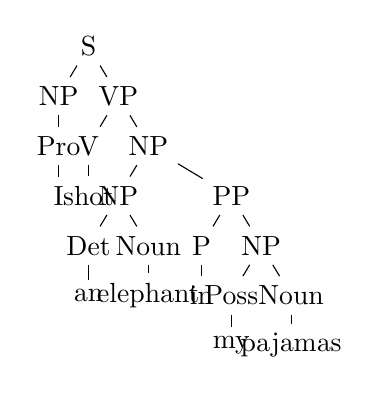
\begin{tikzpicture}[level distance=1.5pc,sibling distance=1.8pc]
    \node {S}
      child {node {NP}
        child {node {Pro}
          child {node {\upshape I}}
        }
      }
      child {node {\alert{VP}}
        child {node {V} child {node {\upshape shot}}}
        child {node {NP}
          child {node {NP}
            child {node {Det} child {node {\upshape an}}}
            child {node {Noun} child {node {\upshape elephant}}}
          }
          child [sibling distance=5pc] {node {PP}
            child [sibling distance=1.8pc] {node {P} child {node {\upshape in}}}
            child [sibling distance=1.8pc] {node {NP}
              child {node {Poss} child {node {\upshape my}}}
              child {node {Noun} child {node {\upshape pajamas}}}
            }
          }
        }
      }
    ;
  \end{tikzpicture}
\end{minipage}%
\begin{minipage}{0.3\textwidth}
\tiny\itshape
  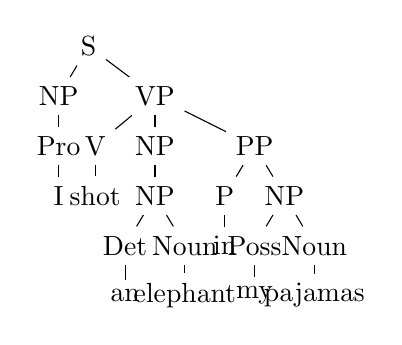
\begin{tikzpicture}[level distance=1.5pc,sibling distance=1.8pc]
    \node {S}
      child {node {NP}
        child {node {Pro}
          child {node {\upshape I}}
        }
      }
      child [sibling distance=4pc] {node {\alert{VP}}
        child [sibling distance=1.8pc] {node {V} child {node {\upshape shot}}}
        child [sibling distance=1.8pc] {node {NP}
          child {node {NP}
            child {node {Det} child {node {\upshape an}}}
            child {node {Noun} child {node {\upshape elephant}}}
          }
        }
        child [sibling distance=3pc] {node {PP}
          child [sibling distance=1.8pc] {node {P} child {node {\upshape in}}}
          child [sibling distance=1.8pc] {node {NP}
            child {node {Poss} child {node {\upshape my}}}
            child {node {Noun} child {node {\upshape pajamas}}}
          }
        }
      }
    ;
  \end{tikzpicture}
\end{minipage}

\tiny Jurafsky and Martin, \emph{Speech and Language Processing}

\end{frame}

\begin{frame}{The Dangling Else Problem}

Who owns the \emph{else}?

\begin{center}\ttfamily
if (a) if (b) c(); else d();
\end{center}

\hfil
Should this be
\hfil
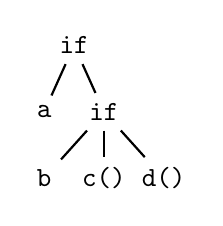
\begin{tikzpicture}[parsetree]
  \node {\texttt{if}}
     child {node {\texttt{a}}}
     child {node {\texttt{if}}
       child {node {\texttt{b}}}
       child {node {\texttt{c()}}}
       child {node {\texttt{d()}}}
     }
  ;
\end{tikzpicture}
\hfil
or
\hfil
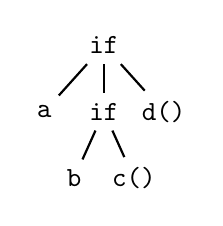
\begin{tikzpicture}[parsetree]
  \node {\texttt{if}}
     child {node {\texttt{a}}}
     child {node {\texttt{if}}
       child {node {\texttt{b}}}
       child {node {\texttt{c()}}}
     }
     child {node {\texttt{d()}}}
  ;
\end{tikzpicture}
\hfil
?

Grammars are usually ambiguous; manuals give disambiguating rules such 
as C's:

\begin{quotation}
\noindent
As usual the ``else'' is resolved by connecting
an else with the last encountered elseless if.
\end{quotation}

\end{frame}

\begin{frame}[fragile]{The Dangling Else Problem}

\begin{ocamlyacc}
stmt : IF expr THEN stmt
     | IF expr THEN stmt ELSE stmt
\end{ocamlyacc}

Problem comes after matching the first statement.  Question is whether
an ``else'' should be part of the current statement or a surrounding
one since the second line tells us ``stmt ELSE'' is possible.

\end{frame}

\begin{frame}[fragile]{The Dangling Else Problem}

Some languages resolve this problem by insisting on nesting
everything.

E.g., Algol 68:

\begin{center}
\begin{algol}
if a < b then a else b fi;
\end{algol}
\end{center}

``fi'' is ``if'' spelled backwards.  The language also uses do--od and
case--esac.
\end{frame}

\begin{frame}[fragile]{Another Solution to the Dangling Else Problem}

Idea: break into two types of statements: those that have a dangling
``then'' (``dstmt'') and those that do not (``cstmt'').  A statement may be
either, but the statement just before an ``else'' must not have a
dangling clause because if it did, the ``else'' would belong to it.

\begin{ocamlyacc}
stmt : dstmt
     | cstmt

dstmt : IF expr THEN stmt
      | IF expr THEN cstmt ELSE dstmt

cstmt : IF expr THEN cstmt ELSE cstmt
      | other statements...
\end{ocamlyacc}

We are effectively carrying an extra bit of information during
parsing: whether there is an open ``then'' clause.  Unfortunately,
duplicating rules is the only way to do this in a context-free grammar.

\end{frame}

\begin{frame}{Ambiguous Arithmetic}

Ambiguity can be a problem in expressions.  Consider parsing

\begin{center}
\texttt{3 - 4 * 2 + 5}
\end{center}

with the grammar

\[e \rightarrow  e + e | e - e | e * e | e \mathop{/} e | N\]

\ttfamily

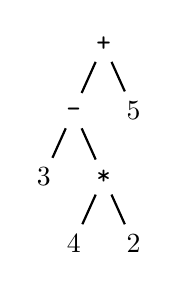
\begin{tikzpicture}[parsetree]
  \path
    \plus{\minus{\lit3}
                {\mult{\lit4}{\lit2}}}
         {\lit5}
    ;
\end{tikzpicture}
\hfil
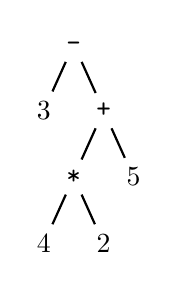
\begin{tikzpicture}[parsetree]
  \path
    \minus{\lit3}
          {\plus{\mult{\lit4}{\lit2}}
                {\lit5}}
    ;
\end{tikzpicture}
\hfil
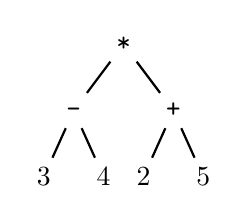
\begin{tikzpicture}[parsetree,
                 level 1/.style={sibling distance=3pc},
                 level 2/.style={sibling distance=1.8pc}]
  \path \mult{\minus{\lit3}{\lit4}}
              {\plus{\lit2}{\lit5}}
    ;
\end{tikzpicture}
\hfil
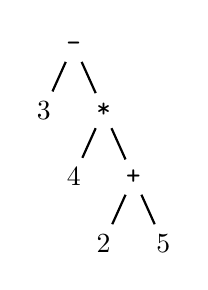
\begin{tikzpicture}[parsetree]
  \path \minus{\lit3}
              {\mult{\lit4}
                     {\plus{\lit2}{\lit5}}};
\end{tikzpicture}
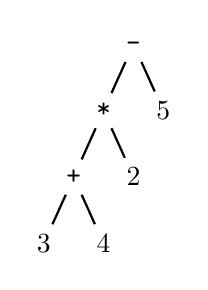
\begin{tikzpicture}[parsetree]
  \path \minus{\mult{\plus{\lit3}{\lit4}}{\lit2}}{\lit5};
\end{tikzpicture}


\end{frame}

\begin{frame}{Operator Precedence and Associativity}

Usually resolve ambiguity in arithmetic expressions

Like you were taught in elementary school:

``My Dear Aunt Sally''

Mnemonic for multiplication and division before addition and subtraction.

\end{frame}

\begin{frame}{Operator Precedence}

Defines how ``sticky'' an operator is.

\begin{center}\ttfamily
1 * 2 + 3 * 4
\end{center}

\begin{minipage}{0.65\textwidth}
\texttt{*} at higher precedence than \texttt{+}:

\medskip

\texttt{(1 * 2) + (3 * 4)}
\end{minipage}
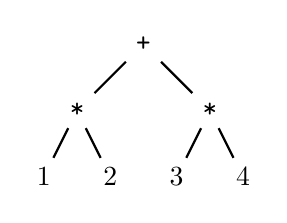
\begin{tikzpicture}[parsetree,
    level 1/.style={sibling distance=4pc},
    level 2/.style={sibling distance=2pc}]
  \path
  \plus{\mult{\lit1}{\lit2}}
       {\mult{\lit3}{\lit4}};
\end{tikzpicture}

\begin{minipage}{0.65\textwidth}
\texttt{+} at higher precedence than \texttt{*}:

\medskip

\texttt{1 * (2 + 3) * 4}
\end{minipage}
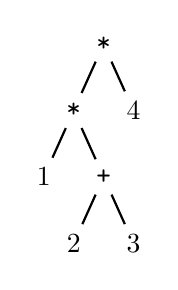
\begin{tikzpicture}[parsetree]
  \path
  \mult{\mult{\lit1}
               {\plus{\lit2}{\lit3}}}
        {\lit4};
\end{tikzpicture}
\end{frame}

\begin{frame}{Associativity}

Whether to evaluate left-to-right or right-to-left

Most operators are left-associative

\begin{center}
\texttt{1 - 2 - 3 - 4}

\vspace{2pc}

\begin{tabular}{c@{\hspace{5pc}}c}
  \ttfamily
  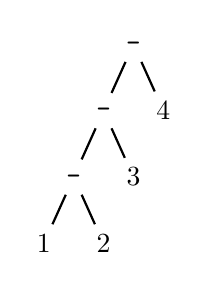
\begin{tikzpicture}[parsetree]
    \path \minus{\minus{\minus{\lit1}{\lit2}}{\lit3}}{\lit4};
  \end{tikzpicture}
&
  \ttfamily
  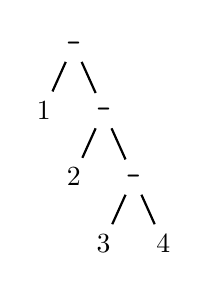
\begin{tikzpicture}[parsetree]
    \path \minus{\lit1}{\minus{\lit2}{\minus{\lit3}{\lit4}}};
  \end{tikzpicture}
\\
\\
$((1 - 2) - 3) - 4$ & $1 - (2 - (3 - 4))$ \\
\\
left associative & right associative
\end{tabular}

\end{center}

\end{frame}

\begin{frame}[fragile]{Fixing Ambiguous Grammars}

A grammar specification:

\begin{ocamlyacc}
expr :
    expr PLUS expr  
  | expr MINUS expr 
  | expr TIMES expr 
  | expr DIVIDE expr
  | NUMBER          
\end{ocamlyacc}

Ambiguous: no precedence or associativity.

Ocamlyacc's complaint: ``16 shift/reduce conflicts.''

\end{frame}

\begin{frame}[fragile]{Assigning Precedence Levels}

Split into multiple rules, one per level

\begin{ocamlyacc}
expr : expr PLUS expr  
     | expr MINUS expr 
     | term            

term : term TIMES term 
     | term DIVIDE term
     | atom            

atom  : NUMBER         
\end{ocamlyacc}

Still ambiguous: associativity not defined

Ocamlyacc's complaint: ``8 shift/reduce conflicts.''

\end{frame}

\begin{frame}[fragile]{Assigning Associativity}

Make one side the next level of precedence

\begin{ocamlyacc}
expr : expr PLUS term  
     | expr MINUS term 
     | term            

term : term TIMES atom 
     | term DIVIDE atom
     | atom            

atom  : NUMBER         
\end{ocamlyacc}

This is left-associative.

No shift/reduce conflicts.

\end{frame}


\begin{frame}[fragile]{Statement separators/terminators}

C uses \texttt{;} as a statement terminator.

\begin{C}
if (a<b)
  printf("a less");
else {
  printf("b"); printf(" less");
}
\end{C}

Pascal uses \texttt{;} as a statement separator. 

\begin{pascal}
if a < b then
  writeln('a less')
else begin
  write('a'); writeln(' less')
end
\end{pascal}

Pascal later made a final \texttt{;} optional.

\end{frame}

\begin{frame}[fragile]{Ocamlyacc Specifications}

\begin{ocamlyacc}
%{
  (* Header: verbatim OCaml; optional *)
%}

  /* Declarations: tokens, precedence, etc. */

%%

  /* Rules: context-free rules */

%%

  (* Trailer: verbatim OCaml; optional *)

\end{ocamlyacc}

\end{frame}

\begin{frame}[fragile]{Declarations}

\parskip=1pc

\begin{itemize}
\item \verb|%token| \emph{symbol} \ldots

 Define symbol names (exported to .mli file)

\item \verb|%token| \verb|<| \emph{type} \verb|>| \emph{symbol} \ldots

 Define symbols with attached attribute (also exported)

\item \verb|%start| \emph{symbol} \ldots

Define start symbols (entry points)

\item \verb|%type| \verb|<| \emph{type} \verb|>| \emph{symbol} \ldots

Define the type for a symbol (mandatory for start)

\item \verb|%left| \emph{symbol} \ldots

\item \verb|%right| \emph{symbol} \ldots

\item \verb|%nonassoc| \emph{symbol} \ldots

Define predecence and associtivity for the given symbols, listed in
order from lowest to highest precedence
\end{itemize}

\end{frame}

\begin{frame}[fragile]{Rules}

\begin{shadedverbatim}
\emph{nonterminal} :
    \emph{symbol} \ldots \emph{symbol} \char`\{ \emph{semantic-action} \}
  | \ldots
  | \emph{symbol} \ldots \emph{symbol} \char`\{ \emph{semantic-action} \}
\end{shadedverbatim}

\begin{itemize}
\item \emph{nonterminal} is the name of a rule, e.g., ``program,'' ``expr''
\item \emph{symbol} is either a terminal (token) or another rule
\item \emph{semantic-action} is OCaml code evaluated when the rule is
  matched
\item In a \emph{semantic-action}, \verb|$1|, \verb|$2|, \ldots returns
  the value of the first, second, \ldots symbol matched
\item A rule may include ``\verb|%prec| \emph{symbol}'' to override
                                its default precedence
\end{itemize}

\end{frame}

\begin{frame}[fragile]{An Example .mly File}

\begin{ocamlyacc}
%token <int> INT
%token PLUS MINUS TIMES DIV LPAREN RPAREN EOL

%left PLUS MINUS /* lowest precedence */
%left TIMES DIV
%nonassoc UMINUS /* highest precedence */

%start main      /* the entry point */
%type <int> main

%%

main:
    expr EOL                { $1 }

expr:
    INT                     { $1 }
  | LPAREN expr RPAREN      { $2 }
  | expr PLUS expr          { $1 + $3 }
  | expr MINUS expr         { $1 - $3 }
  | expr TIMES expr         { $1 * $3 }
  | expr DIV expr           { $1 / $3 }
  | MINUS expr %prec UMINUS { - $2 }
\end{ocamlyacc}

\end{frame}

\part{Parsing Algorithms}
\frame{\partpage}

\begin{frame}{Parsing Context-Free Grammars}

There are $O(n^3)$ algorithms for parsing arbitrary CFGs, but most
compilers demand $O(n)$ algorithms.

\medskip

Fortunately, the LL and LR subclasses of CFGs have $O(n)$ parsing
algorithms.  People use these in practice.

\end{frame}

\if 0

%token PLUS TIMES ID
%start e
%type <int>e

%%

e : t PLUS e { 0 }
  | t        { 0 }

t : ID TIMES t { 0 }
  | ID         { 0 }

ocamlyacc -v lrexample.mly

   0  $accept : %entry% $end

   1  e : t PLUS e
   2    | t

   3  t : ID TIMES t
   4    | ID

   5  %entry% : '\001' e

state 0
	$accept : . %entry% $end  (0)

	'\001'  shift 1
	.  error

	%entry%  goto 2


state 1
	%entry% : '\001' . e  (5)

	ID  shift 3
	.  error

	e  goto 4
	t  goto 5


state 2
	$accept : %entry% . $end  (0)

	$end  accept


state 3
	t : ID . TIMES t  (3)
	t : ID .  (4)

	TIMES  shift 6
	$end  reduce 4
	PLUS  reduce 4


state 4
	%entry% : '\001' e .  (5)

	.  reduce 5


state 5
	e : t . PLUS e  (1)
	e : t .  (2)

	PLUS  shift 7
	$end  reduce 2


state 6
	t : ID TIMES . t  (3)

	ID  shift 3
	.  error

	t  goto 8


state 7
	e : t PLUS . e  (1)

	ID  shift 3
	.  error

	e  goto 9
	t  goto 5


state 8
	t : ID TIMES t .  (3)

	.  reduce 3


state 9
	e : t PLUS e .  (1)

	.  reduce 1


6 terminals, 4 nonterminals
6 grammar rules, 10 states

\fi

% $

\newsavebox{\rightmostDerivation}
\begin{lrbox}{\rightmostDerivation}
  \begin{tikzpicture}[every node/.style={anchor=base,inner sep=2pt},
                      node distance=0pt]
  \node (t1) {$e$};
  \node [below=of t1,matrix of math nodes,inner sep=0pt] (t2) {
    t & + & |(t3)| e \\ };
  \node [below=of t2,matrix of math nodes] (t4) {
    t & + & |(t5)| t \\ };
  \node [below=of t4,matrix of math nodes] (t6) {
    |(t8)| t & + & |(t7)| \id \\ };
  \node [below=of t6,matrix of math nodes] (t9) {
    |(t10)| \id & * & |(t10a)| t & + & \id \\ };
  \node [below=of t9,matrix of math nodes] (t11) {
    \id & * & |(t12)| \id & + & \id \\ };
  \begin{pgfonlayer}{background}
    \expand{t1}{t2}{t2}
    \expand{t3}{t5}{t5}
    \expand{t5}{t7}{t7}
    \expand{t8}{t10}{t10a}
    \expand{t10a}{t12}{t12}
  \end{pgfonlayer}
      \end{tikzpicture}
\end{lrbox}

\begin{frame}[t,fragile]{Rightmost Derivation of $\id * \id + \id$}

\begin{columns}
  \begin{column}{0.3\textwidth}
    \grammarone
  \end{column}
  \begin{column}{0.7\textwidth}

\begin{center}
\begin{tikzpicture}[every node/.style={anchor=base,inner sep=2pt},
  node distance=0.3pc]
  \node (t1) {$e$};
  \pause
  \node [below=of t1,matrix of math nodes,inner sep=0pt] (t2) {
    t & + & |(t3)| e \\ };
  \pause
  \node [below=of t2,matrix of math nodes] (t4) {
    t & + & |(t5)| t \\ };
  \pause
  \node [below=of t4,matrix of math nodes] (t6) {
    |(t8)| t & + & |(t7)| \id \\ };
  \pause
  \node [below=of t6,matrix of math nodes] (t9) {
    |(t10)| \id & * & |(t10a)| t & + & \id \\ };
  \pause
  \node [below=of t9,matrix of math nodes] (t11) {
    \id & * & |(t12)| \id & + & \id \\ };
  \begin{pgfonlayer}{background}
    \onslide<2->{\expand{t1}{t2}{t2}}
    \onslide<3->{\expand{t3}{t5}{t5}}
    \onslide<4->{\expand{t5}{t7}{t7}}
    \onslide<5->{\expand{t8}{t10}{t10a}}
    \onslide<6->{\expand{t10a}{t12}{t12}}
  \end{pgfonlayer}
\end{tikzpicture}
\end{center}
  \end{column}
\end{columns}

\begin{center}

At each step, expand the \emph{rightmost} nonterminal.

\vspace{0.5pc}

\begin{tikzpicture}[node distance=0.5pc]
  \node (nt) {nonterminal};
  \node [below=of nt] (h)
        {``handle'': The right side of a production};
  \begin{pgfonlayer}{background}
    \expand{nt}{h}{h}
  \end{pgfonlayer}
\end{tikzpicture}

\only<1-6>{
Fun and interesting fact: there is exactly one rightmost expansion if
the grammar is unambigious.
}

\only<7>{
Dragon-book style: underline handles

$e
\rightarrow
\underline{t + e}
\rightarrow
t + \underline{t}
\rightarrow
t + \underline{\id}
\rightarrow 
\underline{\id * t} + \id
\rightarrow 
\id * \underline{\id} + \id
$
}

\end{center}

\end{frame}

\begin{frame}[t,fragile]{Rightmost Derivation: What to Expand}

\begin{columns}
  \begin{column}{0.3\textwidth}
    \grammarone
  \end{column}
  \begin{column}{0.7\textwidth}
    \begin{center}
      \usebox{\rightmostDerivation}
    \end{center}
  \end{column}
\end{columns}

\begin{center}
  \begin{tikzpicture}[every node/.style={inner sep=2pt}]
  \node [anchor=east] (t1) {$e$};
  \node [anchor=east,matrix of math nodes,inner sep=0pt] at (0,-1.5pc) (t2) {
    t & + & |(t3)| e \\ };
  \node [anchor=east,matrix of math nodes] at (0,-3pc) (t4) {
    t & + & |(t5)| t \\ };
  \node [anchor=t8.east,matrix of math nodes] at (0,-4.5pc) (t6) {
    |(t8)| t & + & |(t7)| \id \\ };
  \node [anchor=t10a.east,matrix of math nodes] at (0,-6pc) (t9) {
    |(t10)| \id & * & |(t10a)| t & + & \id \\ };
  \node [anchor=west,matrix of math nodes] at (0,-7.5pc) (t11) {
    \id & * & |(t12)| \id & + & \id \\ };
  \begin{pgfonlayer}{background}
    \fill [black!10] (t1.north east) [rounded corners] rectangle +(-6pc,-9pc)
          node [black,below right] {Expand here $\uparrow$};
    \fill [black!10] ($(t1.north east) + (2pt,0)$)
          [rounded corners] rectangle +(6pc,-9pc)
          node [black,below] {Terminals only};
    \expand{t1}{t2}{t2}
    \expand{t3}{t5}{t5}
    \expand{t5}{t7}{t7}
    \expand{t8}{t10}{t10a}
    \expand{t10a}{t12}{t12}
  \end{pgfonlayer}
  \end{tikzpicture}
\end{center}

\end{frame}

\begin{frame}[t,fragile]{Reverse Rightmost Derivation}

\begin{columns}
  \begin{column}{0.3\textwidth}
    \grammarone
  \end{column}
  \begin{column}{0.7\textwidth}
    \begin{center}
      \usebox{\rightmostDerivation}
    \end{center}
  \end{column}
\end{columns}

\begin{center}
  \begin{tikzpicture}[every node/.style={inner sep=1pt}]
  \node [anchor=west,matrix of math nodes] at (0,0) (t11) {
    \id & * & |(t12)| \id & + & \id \\ };
  \pause
  \node (h10) at (9.8pc,0pc) {\id};
  \node (h9) at (9.8pc,-1.5pc) {$t$};
  \draw (h10) to (h9);
  \node [anchor=t10a.east,matrix of math nodes] at (0,-1.5pc) (t9) {
    |(t10)| \id & * & |(t10a)| t & + & \id \\ };
  \pause
  \node (h8) at (8.8pc,-1.5pc) {$*$};
  \node (h7) at (7.8pc,-1.5pc) {\id};
  \node (h6) at (8.8pc,-3pc) {$t$};
  \draw (h6) to (h7)
        (h6) to (h8)
        (h6) to (h9);
  \node [anchor=t8.east,matrix of math nodes] at (0,-3pc) (t6) {
    |(t8)| t & + & |(t7)| \id \\ };
  \pause
  \node (h5) at (10.6pc,-3pc) {\id};
  \node (h4) at (10.6pc,-4.5pc) {$t$};
  \draw (h4) to (h5);
  \node [anchor=east,matrix of math nodes] at (0,-4.5pc) (t4) {
    t & + & |(t5)| t \\ };
  \pause
  \node (h3) at (10.6pc,-6pc) {$e$};
  \draw (h3) to (h4);
  \node [anchor=east,matrix of math nodes] at (0,-6pc) (t2) {
    t & + & |(t3)| e \\ };
  \pause
  \node (h1) at (8.8pc,-7.5pc) {$e$};
  \node (h2) at (9.6pc,-6pc) {$+$};
  \draw (h1) to (h2)
        (h1) to (h3)
        (h1) to (h6);
  \node [anchor=east] (t1) at (0,-7.5pc) {$e$};
  \begin{pgfonlayer}{background}
    \fill [black!10] (t11.north west) [rounded corners] rectangle +(-6pc,-9pc)
          node [black,below right] {viable prefixes};
    \fill [black!10] ($(t11.north west) + (2pt,0)$)
          [rounded corners] rectangle +(6pc,-9pc)
          node [black,below left] {terminals};
    \onslide<6->{\expandup{t1}{t2}{t2}}
    \onslide<5->{\expandup{t3}{t5}{t5}}
    \onslide<4->{\expandup{t5}{t7}{t7}}
    \onslide<3->{\expandup{t8}{t10}{t10a}}
    \onslide<2->{\expandup{t10a}{t12}{t12}}
  \end{pgfonlayer}
  \end{tikzpicture}
\end{center}

\end{frame}

\begin{frame}[fragile,t]{Shift/Reduce Parsing Using an Oracle}

\begin{columns}
  \begin{column}{0.3\textwidth}
    \grammarone
  \end{column}
  \begin{column}{0.7\textwidth}
    \begin{center}
      \usebox{\rightmostDerivation}
    \end{center}
  \end{column}
\end{columns}

\begin{center}
  \begin{tikzpicture}[every node/.style={inner sep=1pt}]
  \node [anchor=west,matrix of math nodes] at (0,0) (t0) {
    \id & * & \id & + & \id \\ };
  \node [anchor=west] at (6.5pc,0pc) {shift};
  \pause
  \node [anchor=t1.east,matrix of math nodes] at (0,-1pc) {
    |(t1)| \id & * & \id & + & \id \\ };
  \node [anchor=west] at (6.5pc,-1pc) {shift};
  \pause
  \node [anchor=t2.east,matrix of math nodes] at (0,-2pc) {
    \id & |(t2)| * & \id & + & \id \\ };
  \node [anchor=west] at (6.5pc,-2pc) {shift};
  \pause
  \node [anchor=t3.east,matrix of math nodes] at (0,-3pc) {
    \id & * &  |(t3)| \id & + & \id \\ };
  \node [anchor=west] at (6.5pc,-3pc) {reduce 4};
  \pause
  \node [anchor=t4.east,matrix of math nodes] at (0,-4pc) {
    |(t5)| \id & * &  |(t4)| t & + & \id \\ };
  \node [anchor=west] at (6.5pc,-4pc) {reduce 3};
  \pause
  \node [anchor=t6.east,matrix of math nodes] at (0,-5pc) {
    |(t6)| t & + & \id \\ };
  \node [anchor=west] at (6.5pc,-5pc) {shift};
  \pause
  \node [anchor=t7.east,matrix of math nodes] at (0,-6pc) {
    t & |(t7)| + & \id \\ };
  \node [anchor=west] at (6.5pc,-6pc) {shift};
  \pause
  \node [anchor=t8.east,matrix of math nodes] at (0,-7pc) {
    t & + & |(t8)| \id \\ };
  \node [anchor=west] at (6.5pc,-7pc) {reduce 4};
  \pause
  \node [anchor=t9.east,matrix of math nodes] at (0,-8pc) {
    t & + & |(t9)| t \\ };
  \node [anchor=west] at (6.5pc,-8pc) {reduce 2};
  \pause
  \node [anchor=t10.east,matrix of math nodes] at (0,-9pc) {
    |(t11)| t & + & |(t10)| e \\ };
  \node [anchor=west] at (6.5pc,-9pc) {reduce 1};
  \pause
  \node [anchor=east] at (0,-10pc) (t12) {$e$};
  \node [anchor=west] at (6.5pc,-10pc) {accept};
  \begin{pgfonlayer}{background}
    \fill [black!10] (t0.north west) [rounded corners] rectangle +(-6pc,-11pc)
          node [black,below right] {stack};
    \fill [black!10] ($(t0.north west) + (2pt,0)$)
          [rounded corners] rectangle +(6pc,-11pc)
          node [black,below left] {input};
    \onslide<5->{\expandup{t4}{t3}{t3}}
    \onslide<6->{\expandup{t6}{t5}{t4}}
    \onslide<9->{\expandup{t9}{t8}{t8}}
    \onslide<10->{\expandup{t10}{t9}{t9}}
    \onslide<11->{\expandup{t12}{t11}{t10}}
  \end{pgfonlayer}
  \end{tikzpicture}
\end{center}

\end{frame}

\begin{frame}{Handle Hunting}

\textbf{Right Sentential Form:} any step in a rightmost derivation

\textbf{Handle:} in a sentential form, a RHS of a rule that, when
rewritten, yields the previous step in a rightmost derivation.

The big question in shift/reduce parsing:

\begin{center}
When is there a handle on the top of the stack?
\end{center}

Enumerate all the right-sentential forms and pattern-match against
them? \emph{Usually infinitely many; let's try anyway.}

\end{frame}

\newcommand{\handle}[3]{$#1\underline{#2}#3$}

\begin{frame}[t]{Some Right-Sentential Forms and Their Handles}
\vbox to 7pc{
  \vrule height 20pt depth 4pt width 0pt
  \grammarone
  \vss
}
{
\footnotesize
\begin{tikzpicture}[level distance=1.5pc,
  inner sep=1pt,
  level 1/.style={sibling distance=12pc},
  level 2/.style={sibling distance=2pc},
  level 3/.style={sibling distance=3pc},
  level 4/.style={sibling distance=3pc},
  level 5/.style={sibling distance=4.5pc},
  level 6/.style={sibling distance=6pc},
  ]
  \node {$e$}
    child {node {\handle{}{t}{}}
      child {node {\handle{}{\id * t}{}}
        child {node {\handle{\id *}{\id * t}{}}
          child [sibling distance=4pc] {node {\handle{\id * \id *}{\id * t}{}}
            child [sibling distance=1pc]
            child [sibling distance=1pc]
          }
          child [sibling distance=5pc] {node {\handle{\id * \id *}{\id}{}}}
        }
        child {node {\handle{\id * }{\id}{}}}
      }
      child {node {\handle{}{\id}{}}}
    }
    child
  ;
\end{tikzpicture}
}
\end{frame}

\begin{frame}[t]{Some Right-Sentential Forms and Their Handles}
\vbox to 7pc{
  \vrule height 20pt depth 4pt width 0pt
  \grammarone
  \vss
}
{
\footnotesize
\begin{tikzpicture}[level distance=1.5pc,
  inner sep=1pt,
  level 1/.style={sibling distance=12pc},
  level 2/.style={sibling distance=2pc},
  level 3/.style={sibling distance=3pc},
  level 4/.style={sibling distance=3pc},
  level 5/.style={sibling distance=4.5pc},
  level 6/.style={sibling distance=6pc},
  ]
  \node {$e$}
    child {node {\handle{}{t}{}}
      child {node {\handle{}{\id * t}{}}
        child {node {\handle{\id *}{\id * t}{}}
          child [sibling distance=4pc] {node {\handle{\id * \id *}{\id * t}{}}
            child [sibling distance=1pc]
            child [sibling distance=1pc]
          }
          child [sibling distance=5pc] {node {\handle{\id * \id *}{\id}{}}}
        }
        child {node {\handle{\id * }{\id}{}}}
      }
      child {node {\handle{}{\id}{}}}
    }
    child {node {\handle{}{t+e}{}}
      child [sibling distance=12pc] {node {\handle{t+}{t+e}{}}
        child {node {\handle{t+t+}{t+e}{}}
          child [sibling distance=2pc]
          child [sibling distance=2pc] {node {\handle{t+t+t+}{t}{}}
            child [sibling distance=1pc]
            child [sibling distance=1pc]
          }
        }
        child [sibling distance=1pc]
      }
      child
    }
  ;
\end{tikzpicture}
}
\end{frame}

\newcommand{\sentineltree}{
\footnotesize
\begin{tikzpicture}[level distance=1.5pc,
  inner sep=1pt,
  level 1/.style={sibling distance=12pc},
  level 2/.style={sibling distance=2pc},
  level 3/.style={sibling distance=3pc},
  level 4/.style={sibling distance=3pc},
  level 5/.style={sibling distance=4.5pc},
  level 6/.style={sibling distance=6pc},
  ]
  \node {$e$}
    child {node {\handle{}{t}{}}
      child {node {\handle{}{\id * t}{}}
        child {node {\handle{\id *}{\id * t}{}}
          child [sibling distance=4pc] {node {\handle{\id * \id *}{\id * t}{}}
            child [sibling distance=1pc]
            child [sibling distance=1pc]
          }
          child [sibling distance=5pc] {node {\handle{\id * \id *}{\id}{}}}
        }
        child {node {\handle{\id * }{\id}{}}}
      }
      child {node {\handle{}{\id}{}}}
    }
    child {node {\handle{}{t+e}{}}
      child [sibling distance=12pc] {node {\handle{t+}{t+e}{}}
        child {node {\handle{t+t+}{t+e}{}}
          child [sibling distance=2pc]
          child [sibling distance=2pc] {node {\handle{t+t+t+}{t}{}}
            child [sibling distance=1pc]
            child [sibling distance=1pc]
          }
        }
        child [sibling distance=1pc]
      }
      child {node {\handle{t+}{t}{}}
        child [sibling distance=6pc] {node {\handle{t+}{\id*t}{}}
          child [sibling distance=1pc]
          child [sibling distance=1pc]
        }
        child {node {\handle{t+}{\id}{}}
          child {node {\handle{}{\id * t}{+ \id}}
            child {node {\handle{\id * }{\id * t}{ + \id}}
              child {node {\handle{\id * \id * }{\id * t}{ + \id}}
                child [sibling distance=1pc]
                child [sibling distance=1pc]
              }
              child {node {\handle{\id * \id * }{\id}{ + \id}}}
            }
            child {node {\handle{\id * }{\id}{+ \id}}}
          }
          child {node {\handle{}{\id}{ + \id}}}
        }        
%        child {node {\handle{\id * }{\id}{}}}
      }
    }
  ;
\end{tikzpicture}
}

\newsavebox{\automataPatterns}
\begin{lrbox}{\automataPatterns}
\footnotesize%\renewcommand{\arraystretch}{0.1}
\begin{tabular}[t]{l}
\handle{\id * \id * \cdots * }{\id * t}{\cdots} \\
\handle{\id * \id * \cdots * }{\id}{\cdots} \\
\handle{t + t + \cdots + }{t+e}{} \\
\handle{t + t + \cdots + t + }{\id}{} \\
\handle{t + t + \cdots + t + \id * \id * \cdots * }{\id * t}{} \\
\handle{t + t + \cdots + }{t}{} \\
e \\
\end{tabular}
\end{lrbox}

\begin{frame}[t]{Some Right-Sentential Forms and Their Handles}
\vbox to 7pc{
  \vrule height 20pt depth 4pt width 0pt
  \grammarone
  \hfill
  Patterns: \usebox{\automataPatterns}
  \vss
}
\sentineltree
\end{frame}

\begin{frame}{The Handle-Identifying Automaton}

Magical result, due to Knuth:  \emph{An automaton suffices to locate a handle
  in a right-sentential form.}

\begin{columns}
  \begin{column}{0.6\textwidth}
    \usebox{\automataPatterns}
  \end{column}
  \begin{column}{0.4\textwidth}
\begin{tikzpicture}[node distance=1.2pc and 2pc,initial text={},
    every state/.style={minimum size=28pt}]
  \node [state,initial] (S0) {};
  \node [state,below=of S0,accepting] (S1) {$\id$};
  \node [state,right=of S0,accepting] (S2) {$t$};
  \node [state,below=of S1] (S3) {};
  \node [state,below=of S2] (S4) {};
  \node [state,below=of S3,accepting] (S5) {$\id * t$};
  \node [state,below=of S4,accepting] (S6) {$t + e$};
  \node [state,above=of S0,accepting] (S7) {$e$};
  \path [->]
     (S0) edge node [above] {$t$} (S2)
     (S2) edge [bend left] node [right] {$+$} (S4)
     (S4) edge [bend left] node [left] {$t$} (S2)
     (S4) edge node [right] {$e$} (S6)
     (S4) edge node [above] {$\id$} (S1)
     (S0) edge node [right] {$\id$} (S1)   
     (S1) edge [bend left] node [right] {$*$} (S3)
     (S3) edge [bend left] node [left] {$\id$} (S1)
     (S3) edge node [right] {$t$} (S5)
     (S0) edge node [right] {$e$} (S7)
  ;
\end{tikzpicture}
  \end{column}
\end{columns}

\end{frame}

\begin{frame}{Building the Initial State of the LR(0) Automaton}
\parskip=2pt

\mbox{}
%\vspace{0.5\baselineskip}

\begin{columns}
  \begin{column}{0.5\textwidth}
    \grammarone
  \end{column}
  \begin{column}{0.5\textwidth}
    \framebox{$\begin{array}{l}
    e' \rightarrow \pac e \\
    \onslide<2->{e \rightarrow \pac t + e \\
    e \rightarrow \pac t \\}
    \onslide<3->{t \rightarrow \pac \id * t \\
    t \rightarrow \pac \id}
  \end{array}$
    }
  \end{column}
\end{columns}

Key idea: automata identify viable prefixes of right sentential forms.
Each state is an equivalence class of possible places in productions.

At the beginning, any viable prefix must be at the beginning of a
string expanded from $e$.  We write this condition ``$e' \rightarrow
\pac e$''

\onslide<2->{There are two choices for what an $e$ may expand to:
  $t+e$ and $t$.  So when $e' \rightarrow \pac e$, $e \rightarrow \pac
  t+e$ and $e \rightarrow \pac t$ are also true, i.e., it must start
  with a string expanded from $t$.}

\onslide<3->{Also, $t$ must be $\id * t$ or $\id$, so $t
  \rightarrow \pac \id * t$ and $t \rightarrow \pac \id$.

This is a \emph{closure}, like $\epsilon$-closure
in subset construction.
}

\end{frame}

\begin{frame}{Building the LR(0) Automaton}

\begin{columns}
  \begin{column}{0.5\textwidth}
\small
\begin{tikzpicture}[node distance=1.5pc]

  \node [draw] (S0) {$\textbf{S0}: \begin{array}{@{}l@{}}
    e' \rightarrow \pac e \\
    e \rightarrow \pac t + e \\
    e \rightarrow \pac t \\
    t \rightarrow \pac \id * t \\
    t \rightarrow \pac \id
  \end{array}$};

  \onslide<2->{

    \node [draw,accepting,below=of S0] (S1) {$\textbf{S1}: \begin{array}{@{}l@{}}
        t \rightarrow \id \pac * t \\
        t \rightarrow \id \pac
      \end{array}$};

    \node [draw,accepting,above=of S0] (S7) {$\textbf{S7}:\ e'
      \rightarrow e \pac$};

    \node [draw,accepting,right=of S0] (S2) {$\textbf{S2}: \begin{array}{@{}l@{}}
        e \rightarrow t \pac + e \\
        e \rightarrow t \pac
      \end{array}$};

     \path [->]
     (S0) edge node [right] {$e$} (S7)
     (S0) edge node [right] {$\id$} (S1)
     (S0) edge node [above] {$t$} (S2)
     ;
  }

  \onslide <3->{
    \node [draw,below=of S1] (S3) {$\textbf{S3}: \begin{array}{@{}l@{}}
        t \rightarrow \id * \pac t \\
        \onslide<4->{
        t \rightarrow \pac \id * t \\
        t \rightarrow \pac \id}
      \end{array}$};

    \node [draw,right=of S2] (S4)
          {$\textbf{S4}: \begin{array}{@{}l@{}}
              e \rightarrow t + \pac e \\
              \onslide<4->{
              e \rightarrow \pac t + e \\
              e \rightarrow \pac t \\
              t \rightarrow \pac \id * t \\
              t \rightarrow \pac \id}
            \end{array}$};

    \path [->] (S1) edge [bend left=10] node [right] {$*$} (S3)
               (S2) edge [bend left=10] node [above] {$+$} (S4);
  }

  \onslide<5->{

    \node [draw,accepting,right=of S3] (S5) {$\textbf{S5}:\ t
      \rightarrow \id * t \pac$};

    \path [->]
      (S3) edge node [above] {$t$} (S5)
      (S3) edge [bend left=10] node [left] {$\id$} (S1);

    \node [draw,accepting, below=of S4] (S6)
          {$\textbf{S6}:\ e \rightarrow t + e \pac$};

    \path [->] (S4) edge [bend left=10] node [below] {$t$} (S2)
      (S4) edge [bend left=10] node [above] {$\id$} (S1)
      (S4) edge node [right] {$e$} (S6);
  }

  \onslide<2>{

    \node [above,text width=6.5pc,text ragged] at (S2.north)
          {\footnotesize\emph{``Just passed a
              prefix ending in a string derived from $t$''}};

    \node [below,text width=8pc,text badly ragged] at (S1.south)
          {\footnotesize\emph{``Just passed a prefix that ended in an \id''}};

    \node [above,text width=8pc,text ragged] at (S7.north)
          {\footnotesize\emph{``Just passed a string derived from $e$''}};
  }
\end{tikzpicture}
  \end{column}
  \begin{column}{0.5\textwidth}
    \onslide<1-2>{%
      The first state suggests a viable prefix can start as any string
      derived from $e$, any string derived from $t$, or $\id$.
      \medskip
    }

    \onslide<2>{
      The items for these three states come from advancing the $\pac$
      across each thing, then performing the closure operation
      (vacuous here).
    }

    \onslide<3-4>{In S2, a $+$ may be next.  This gives $t + \pac e$.
      \onslide<4>{Closure adds 4 more items.}

      \medskip

      In S1, $*$ may be next, giving $\id * \pac t$
      \onslide<4>{and two others.}      
    }
  \end{column}
\end{columns}

\end{frame}

\begin{frame}{What to do in each state?}

\begin{columns}
\begin{column}{0.33\textwidth}
\begin{tikzpicture}[node distance=1.5pc]

    \node [draw,accepting] (S1) {$\textbf{S1}: \begin{array}{@{}l@{}}
        t \rightarrow \id \pac * t \\
        t \rightarrow \id \pac
      \end{array}$};

    \draw [->] (S1) -- node [right] {$*$} ($(down:1.3)$);
    \draw [<-] (S1) -- node [right] {$\id$} ($(up:1.3)$);

\end{tikzpicture}
\end{column}%
\begin{column}{0.23\textwidth}
\grammarone
\end{column}
\begin{column}{0.43\textwidth}
\usebox{\automataPatterns}
\end{column}
\end{columns}

\begin{tabular}{rll}
\toprule
\multicolumn{1}{c}{\textbf{Stack}} & \textbf{Input} & \textbf{Action} \\
\midrule
$\id * \id * \cdots * \id$ & $* \cdots$ & Shift \\
$\id * \id * \cdots * \id$ & $+ \cdots$ & Reduce 4 \\
$\id * \id * \cdots * \id$ & & Reduce 4 \\
$\id * \id * \cdots * \id$ & $\id \cdots$ & Syntax Error \\
\bottomrule
\end{tabular}


\end{frame}

\newcommand\first{\textsc{first}}
\newcommand\follow{\textsc{follow}}

\begin{frame}{The \first{} function}

\parskip=5pt

If you can derive a string that starts with terminal $t$ from a
sequence of terminals and nonterminals $\alpha$, then $t \in
\first(\alpha)$.

\begin{enumerate}
\item If $X$ is a terminal, $\first(X) = \{ X \}$.

\item If $X \rightarrow \epsilon$, then add $\epsilon$ to $\first(X)$.

\item If $X \rightarrow Y_1 \cdots Y_k$ and
  $\epsilon \in \first(Y_1)$,
  $\epsilon \in \first(Y_2)$, \ldots, and $\epsilon \in
  \first(Y_{i-1})$ for $i=1,\ldots, k$ for some $k$, \\ \quad add
  $\first(Y_i) - \{ \epsilon \}$ to $\first(X)$

    \textcolor{red}{\emph{$X$ starts with anything that appears after
      skipping empty strings. Usually just $\first(Y_1) \in \first(X)$}}

\item If $X \rightarrow Y_1 \cdots Y_K$ and
  $\epsilon \in \first(Y_1)$,
  $\epsilon \in \first(Y_2)$, \ldots, and $\epsilon \in \first(Y_k)$, add
  $\epsilon$ to $\first(X)$

    \textcolor{red}{\emph{If all of $X$ can be empty, $X$ can be empty}}  
\end{enumerate}

\hrule

\vspace{5pt}

\begin{columns}
\begin{column}{0.3\textwidth}
\grammarone
\end{column}
\begin{column}{0.7\textwidth}
\parskip=5pt
$\first(\id) = \{ \id \}$

$\first(t) = \{ \id \}$ because $t \rightarrow \id\ * t$ and $t
  \rightarrow \id$

$\first(e) = \{ \id \}$ because $e \rightarrow t + e$, $e \rightarrow
  t$, and $\first(t) = \{ \id \}$.

\end{column}
\end{columns}

\end{frame}

\begin{frame}{First and $\epsilon$}
  $\epsilon \in \first(\alpha)$ means $\alpha$ can derive the empty
  string.

  \begin{enumerate}
\item If $X$ is a terminal, $\first(X) = \{ X \}$.

\item If $X \rightarrow \epsilon$, then add $\epsilon$ to $\first(X)$.

\item If $X \rightarrow Y_1 \cdots Y_k$ and \\
  $\epsilon \in \first(Y_1)$,
  $\epsilon \in \first(Y_2)$, \ldots, and $\epsilon \in
  \first(Y_{i-1})$ \\ for $i=1,\ldots, k$ for some $k$, \\ \quad add
  $\first(Y_i) - \{ \epsilon \}$ to $\first(X)$

\item If $X \rightarrow Y_1 \cdots Y_K$ and \\
  $\epsilon \in \first(Y_1)$,
  $\epsilon \in \first(Y_2)$, \ldots, and $\epsilon \in \first(Y_k)$, \\ \quad add
  $\epsilon$ to $\first(X)$
      \end{enumerate}

  \begin{columns}
    \begin{column}{0.15\textwidth}
      $\begin{array}{l@{\,}l@{\,}l}
        X & \rightarrow & Y Z a \\
        Y & \rightarrow & \\
        Y & \rightarrow & b \\
        Z & \rightarrow & c \\
        Z & \rightarrow & W \\
        W & \rightarrow & \\
        W & \rightarrow & d \\
      \end{array}$
    \end{column}
    \begin{column}{0.85\textwidth}
$\begin{array}{ll}

\first(b) = \{ b \}\quad \first(c) = \{ c \}\quad \first(d) = \{ d \} & (1) \\
  
\first(W) = \{ \epsilon \} \cup \first(d) = \{ \epsilon, d \} & (2, 3) \\

\first(Z) = \first(c) \cup (\first(W) - \{\epsilon\}) \cup \{ \epsilon \} = \{ \epsilon, c, d \} & (3, 3, 4) \\

\first(Y) = \{ \epsilon \} \cup \{ b \} = \{ \epsilon, b \} & (2, 3) \\

\first(X) = (\first(Y) - \{\epsilon\}) \cup (\first(Z) - \{\epsilon\}) \cup \\
 \quad \quad \quad \quad \quad \first(a) = \{a, b, c, d\} & (3, 3, 3) \\
      \end{array}$
    \end{column}
  \end{columns}
  
\end{frame}

\begin{frame}{The \textsc{follow} function}

If $t$ is a terminal, $A$ is a nonterminal, and $\cdots A t \cdots$
can be derived, then $t \in \follow(A)$.

\begin{enumerate}
\item Add \$ (``end-of-input'') to $\follow(S)$ (start symbol).

  \textcolor{red}{\emph{End-of-input comes after the start symbol}}

\item For each prod.\ $\rightarrow \cdots A \alpha$, add
  $\first(\alpha) - \{ \epsilon \}$ to $\follow(A)$.

  \textcolor{red}{\emph{$A$ is followed by the first thing after it}}

\item For each prod.\ $A \rightarrow \cdots B$ or $A \rightarrow
  \cdots B \alpha$ where $\epsilon \in \first(\alpha)$, then add
  everything in $\follow(A)$ to $\follow(B)$.

  \textcolor{red}{\emph{If $B$ appears at the end of a production, it
      can be followed by whatever follows that production}}

\end{enumerate}

\hrule

\vspace{5pt}

\begin{columns}
\begin{column}[t]{0.3\textwidth}
\grammarone

$\first(t) = \{\id\}$

$\first(e) = \{\id\}$
\end{column}
\begin{column}[t]{0.7\textwidth}
$\follow(e) = \{ \$ \}$

$\follow(t) = \{ \uncover<2->{+} \uncover<3->{, \$} \}$

\medskip

\only<1>{%
\emph{1. Because $e$ is the start symbol}
}%
\only<2>{%
\emph{2. Because $e \rightarrow \underbar{t} + e$ and $\first(+) = \{+\}$}
}%
\only<3>{%
\emph{3. Because $e \rightarrow \underline{t}$ and $\$ \in \follow(e)$}
}%
\only<4>{%
Fixed-point reached: applying any rule does not change any set
}

\end{column}
\end{columns}

\end{frame}

\def\highlight<#1>#2{
  {\temporal<#1>{\color{black!30}}{}{\color{black!30}}#2}
}

\def\pac{\cdot}

\begin{frame}[t]{Converting the LR(0) Automaton to an SLR Table}

\begin{columns}
  \begin{column}{0.5\textwidth}
\begin{tikzpicture}[node distance=2pc,initial text={}]
  \highlight<1>{\node [draw,initial] (S0) {\textbf{S0}};}
  \highlight<1,2,4,5>{\node [draw,below=of S0,accepting] (S1)
    {\textbf{S1}: $t \rightarrow \id\pac$};}
  \highlight<1,3,5>{\node [draw,right=of S0,accepting] (S2)
    {\textbf{S2}: $e \rightarrow t\pac$};}
  \highlight<2,4>{\node [draw,below=of S1] (S3) {\textbf{S3}};}
  \highlight<3,5>{\node [draw,below=of S2] (S4) {\textbf{S4}};}
  \highlight<4,6>{\node [draw,below=of S3,accepting] (S5)
        {\textbf{S5}: $t \rightarrow \id * t\pac$};}
  \highlight<5,7>{\node [draw,below=of S4,accepting] (S6)
        {\textbf{S6}: $e \rightarrow t + e\pac$};}
  \highlight<1,8>{\node [draw,above=of S0,accepting] (S7)
        {\textbf{S7}: $e' \rightarrow e\pac$};}
 \highlight<1>{\path [->]
  (S0) edge node [above] {$t$} (S2)
  (S0) edge node [right] {$\id$} (S1)   
  (S0) edge node [right] {$e$} (S7);}
 \highlight<2>{\path [->] (S1) edge [bend left] node [right] {$*$} (S3);}
 \highlight<3>{\path [->] (S2) edge [bend left] node [right] {$+$} (S4);}
 \highlight<4>{\path [->]
   (S3) edge [bend left] node [left] {$\id$} (S1)
   (S3) edge node [right] {$t$} (S5);}
 \highlight<5>{\path [->]
   (S4) edge [bend left] node [left] {$t$} (S2)
   (S4) edge node [right] {$e$} (S6)
   (S4) edge node [above] {$\id$} (S1);}

  \node [right=of S7] {\grammarone};
\end{tikzpicture}

$\follow(e) = \{ \$ \}$

$\follow(t) = \{ +, \$ \}$
  \end{column}
  \begin{column}[t]{0.5\textwidth}
    \small
    \begin{tabular}{c|cccc|cc}
      \toprule
      \multicolumn{1}{c}{\textbf{State}} &
      \multicolumn{4}{c}{\textbf{Action}} &
      \multicolumn{2}{c}{\textbf{Goto}} \\
      \cmidrule(lr){2-5}
      \cmidrule(l){6-7}
      \multicolumn{1}{c}{}
      & \id & $+$ & $*$ & \multicolumn{1}{c}{\$} & $e$ & $t$ \\
      \midrule
             0 & s1 &    &    &    & 7 & 2 \\
\onslide<2->{1 &    & r4 & s3 & r4 &   & }  \\
\onslide<3->{2 &    & s4 &    & r2 &   & }  \\
\onslide<4->{3 & s1 &    &    &    &   & 5} \\
\onslide<5->{4 & s1 &    &    &    & 6 & 2} \\
\onslide<6->{5 &    & r3 &    & r3 &   & }  \\
\onslide<7->{6 &    &    &    & r1 &   & } \\
\onslide<8->{7 &    &    &    & \checkmark & & } \\
      \bottomrule
    \end{tabular}

    \onslide*<1>{
      From S0, shift an $\id$ and go to S1;
      or cross a $t$ and go to S2; or
      cross an $e$ and go to S7.}
    \onslide*<2>{
      From S1, shift a $*$ and go to S3; or, if the next input $\in
      \follow(t)$, reduce by rule 4.}
    \onslide*<3>{
      From S2, shift a $+$ and go to S4; or, if the next input $\in
      \follow(e)$, reduce by rule 2.}
    \onslide*<4>{
      From S3, shift an $\id$ and go to S1; or cross a $t$ and go to
      S5.}
    \onslide*<5>{
      From S4, shift an $\id$ and go to S1; or cross an $e$ or a $t$.}
    \onslide*<6>{
      From S5, reduce using rule 3 if the next symbol $\in \follow(t)$.}
    \onslide*<7>{
      From S6, reduce using rule 1 if the next symbol $\in \follow(e)$.}
    \onslide*<8>{If, in S7, we just crossed an $e$, accept if we are at the
      end of the input.}
  \end{column}
\end{columns}

\end{frame}

\def\st#1#2{\begin{tikzpicture}
    \node [fill=mBlue!30,text width=9pt,text centered,inner sep=0pt,
           font={\fontsize{9}{8}\selectfont},
           minimum height=16pt]
          {$#1$\break #2};
  \end{tikzpicture}}

\newsavebox{\reasonbox}
\newenvironment{reason}
   {\begin{lrbox}{\reasonbox}\begin{minipage}{12pc}\raggedright\parskip=5pt}
   {\end{minipage}\end{lrbox}\vbox to 0pt{\rlap{\usebox{\reasonbox}}\vss}}

\begin{frame}[t]{Shift/Reduce Parsing with an SLR Table}

\begin{columns}
  \begin{column}{0.45\textwidth}
    \grammarone

    \medskip

    \footnotesize
    \begin{tabular}{c|cccc|cc}
      \toprule
      \multicolumn{1}{c}{\textbf{State}} &
      \multicolumn{4}{c}{\textbf{Action}} &
      \multicolumn{2}{c}{\textbf{Goto}} \\
      \cmidrule(lr){2-5}
      \cmidrule(l){6-7}
      \multicolumn{1}{c}{}
      & \id & $+$ & $*$ & \multicolumn{1}{c}{\$} & $e$ & $t$ \\
      \midrule
             0 & s1 &    &    &    & 7 & 2 \\
1 &    & r4 & s3 & r4 &   &   \\
2 &    & s4 &    & r2 &   &   \\
3 & s1 &    &    &    &   & 5 \\
4 & s1 &    &    &    & 6 & 2 \\
5 &    & r3 &    & r3 &   &   \\
6 &    &    &    & r1 &   &  \\
7 &    &    &    & \checkmark & &  \\
      \bottomrule
    \end{tabular}
  
  \end{column}
  \begin{column}{0.55\textwidth}
    \footnotesize
    \begin{tabular}{r|ll}
      \toprule
      \multicolumn{1}{c}{\textbf{Stack}} &
      \multicolumn{1}{c}{\textbf{Input}} & \textbf{Action} \\
      \midrule
  \hspace{42pt}
      \st{ }0 & $\id * \id + \id \, \$$ & Shift, goto 1 \\
      \begin{onlyenv}<1>
        \begin{reason}
          Look at the state on top of the stack and the next input
          token.

          Find the action (shift, reduce, or error) in the table.

          In this case, shift the token onto the stack and mark it with
          state 1.
        \end{reason}
      \end{onlyenv}
\onslide<2->{%
      \st{ }0 \st{\id}1 & $ *\, \id + \id \,\$$ & Shift, goto 3 \\}
      \begin{onlyenv}<2>
        \begin{reason}
          Here, the state is 1, the next symbol is $*$, so shift and
          mark it with state 3.
        \end{reason}
      \end{onlyenv}
\onslide<3->{%
      \st{ }0 \st{\id}1 \st{*}3 & $ \id + \id \,\$$ & Shift, goto 1 \\
      \st{ }0 \st{\id}1 \st{*}3 \st{\id}1 & $ +\, \id \,\$$ & Reduce 4 \\}
      \begin{onlyenv}<3>
        \begin{reason}
          Here, the state is 1, the next symbol is $+$.  The table
          says reduce using rule 4.
        \end{reason}
      \end{onlyenv}
\onslide<4->{%
      \st{ }0 \st{\id}1 \st{*}3 \onslide<1-3,5->{\st{t}5} & $ +\, \id
      \,\$$ & \onslide<5->{Reduce 3} \\}
      \begin{onlyenv}<4>
        \begin{reason}
          Remove the RHS of the rule (the handle: here, just $\id$), observe the
          state on the top of the stack, and consult the ``goto''
          portion of the table.
        \end{reason}
      \end{onlyenv}
      \begin{onlyenv}<5>
        \begin{reason}
          Here, we push a $t$ with state 5.  This effectively ``backs
          up'' the LR(0) automaton and runs it over the newly added
          nonterminal.

          In state 5 with an upcoming $+$, the action is ``reduce 3.''
        \end{reason}
      \end{onlyenv}
\onslide<6->{%
      \st{ }0 \st{t}2 & $ +\, \id \,\$$ & Shift, goto 4 \\}
      \begin{onlyenv}<6>
        \begin{reason}
          This time, we strip off the RHS for rule 3, the handle $\id * t$,
          exposing state 0, so we push a $t$ with state 2.
        \end{reason}
      \end{onlyenv}
\onslide<7->{
      \st{ }0 \st{t}2 \st{+}4 & $ \id \,\$$ & Shift, goto 1 \\
      \st{ }0 \st{t}2 \st{+}4 \st{\id}1 & $\$$ & Reduce 4 \\
      \st{ }0 \st{t}2 \st{+}4 \st{t}2 & $\$$ & Reduce 2 \\
      \st{ }0 \st{t}2 \st{+}4 \st{e}6 & $\$$ & Reduce 1 \\
      \st{ }0 \st{e}7 & $\$$ & Accept} \\
      \bottomrule
    \end{tabular}
  \end{column}
\end{columns}

\end{frame}

\begin{frame}{L, R, and all that}

LR parser: ``Bottom-up parser'': \\
L = Left-to-right scan, R = (reverse) Rightmost derivation

RR parser: R = Right-to-left scan (from end) \\
I called them ``Australian style''; nobody uses these

LL parser: ``Top-down parser'': \\
L = Left-to-right scan: L = (reverse) Leftmost derivation

LR(1): LR parser that considers next token (lookahead of 1)

LR(0): Only considers stack to decide shift/reduce

SLR(1): Simple LR: lookahead from first/follow rules \\
Derived from LR(0) automaton

LALR(1): Lookahead LR(1): fancier lookahead analysis \\
Uses same LR(0) automaton as SLR(1)

Ocamlyacc builds LALR(1) tables.

\end{frame}

\begin{frame}{The Punchline}

This is a tricky, but mechanical procedure.  The Ocamlyacc parser
generator uses a modified version of this technique to generate fast
bottom-up parsers.

You need to understand it to comprehend error messages:

\begin{columns}
  \begin{column}{0.5\textwidth}
\raggedright

Shift/reduce conflicts are caused by a state like

\medskip

$\begin{array}{@{}l@{}}
t \rightarrow \pac\> \textbf{Else}\> s \\
t \rightarrow \pac \\
 \end{array}$

\medskip

If the next token is \textbf{Else}, do you reduce it since
\textbf{Else} may follow a $t$, or shift it?
  \end{column}
  \begin{column}{0.5\textwidth}

\raggedright

Reduce/reduce conflicts are caused by a state like

\medskip

$\begin{array}{@{}l@{}}
t \rightarrow \id * t\> \pac \\
e \rightarrow \id * t\> \pac \\
 \end{array}$

\medskip

Do you reduce by ``$t \rightarrow \id * t$'' or by ``$e \rightarrow \id * t$''?

  \end{column}
\end{columns}
\end{frame}


% http://jsmachines.sourceforge.net/machines/slr.html

\begin{frame}{A Reduce/Reduce Conflict}

\begin{columns}
\begin{column}{0.25\textwidth}
$\begin{array}[t]{@{}l@{\,}r@{\,}c@{\,}l@{}}
1: & a & \rightarrow & \id\ \id \\
2: & a & \rightarrow & b \\
3: & b & \rightarrow & \id\ \id \\
\end{array}$
\end{column}
\begin{column}{0.75\textwidth}
\begin{tikzpicture}[node distance=1.5pc]

\node [draw] (S0) {$\textbf{S0}:\begin{array}{@{}l@{}}
   a' \rightarrow \pac\> a \\
   a \rightarrow \pac\> \id\ \id \\
   a \rightarrow \pac\> b \\
   b \rightarrow \pac\> \id\ \id \\
  \end{array}$};

\node [draw,above=of S0] (S1) {$\textbf{S1}: a' \rightarrow a\ \pac$};

\node [draw,right=of S0] (S2) {$\textbf{S2}: \begin{array}{@{}l@{}}
   a \rightarrow \id\ \pac\ \id \\
   b \rightarrow \id\ \pac\ \id \\
  \end{array}$};

\node [draw,accepting,below=of S0] (S3) {$\textbf{S3}: a \rightarrow b \ \pac$};

\node [draw,fill=mBlue!50,below=of S2,accepting] (S4) {$\textbf{S4}: \begin{array}{@{}l@{}}
   a \rightarrow \id\ \id\ \pac \\
   b \rightarrow \id\ \id\ \pac \\
  \end{array}$};

\draw [->] (S0) -- node [right] {$a$} (S1);
\draw [->] (S0) -- node [above] {$\id$} (S2);
\draw [->] (S0) -- node [right] {$b$} (S3);
\draw [->] (S2) -- node [right] {$\id$} (S4);
\end{tikzpicture}
\end{column}
\end{columns}

\end{frame}

\end{document}

% Local Variables:
% compile-command: "make syntax.pdf"
% End:
